\documentclass{article}
\usepackage{natbib} 

% if you need to pass options to natbib, use, e.g.:
%     \PassOptionsToPackage{numbers, compress}{natbib}
% before loading neurips_2026

% The authors should use one of these tracks.
% Before accepting by the NeurIPS conference, select one of the options below.
% 0. "default" for submission
% \usepackage{neurips_2026}
% \usepackage[preprint]{neurips_2026}
\usepackage{scai}
% eandd
% the "default" option is equal to the "main" option, which is used for the Main Track with double-blind reviewing.
% 1. "main" option is used for the Main Track
%  \usepackage[main]{neurips_2026}
% 2. "position" option is used for the Position Paper Track
%  \usepackage[position]{neurips_2026}
% 3. "eandd" option is used for the Evaluations & Datasets Track
 % \usepackage[eandd]{neurips_2026}
 % if you want to opt-in for a de-anomymized submission (not recommended, but OK):
 %\usepackage[eandd, nonanonymous]{neurips_2026}
% 4. "creativeai" option is used for the Creative AI Track
%  \usepackage[creativeai]{neurips_2026}
% 5. "sglblindworkshop" option is used for the Workshop with single-blind reviewing
 % \usepackage[sglblindworkshop]{neurips_2026}
% 6. "dblblindworkshop" option is used for the Workshop with double-blind reviewing
%  \usepackage[dblblindworkshop]{neurips_2026}

% After being accepted, the authors should add "final" behind the track to compile a camera-ready version.
% 1. Main Track
 % \usepackage[main, final]{neurips_2026}
% 2. Position Paper Track
%  \usepackage[position, final]{neurips_2026}
% 3. Evaluations & Datasets Track
 % \usepackage[eandd, final]{neurips_2026}
% 4. Creative AI Track
%  \usepackage[creativeai, final]{neurips_2026}
% 5. Workshop with single-blind reviewing
%  \usepackage[sglblindworkshop, final]{neurips_2026}
% 6. Workshop with double-blind reviewing
%  \usepackage[dblblindworkshop, final]{neurips_2026}
% Note. For the workshop paper template, both \title{} and \workshoptitle{} are required, with the former indicating the paper title shown in the title and the latter indicating the workshop title displayed in the footnote.
% For workshops (5., 6.), the authors should add the name of the workshop, "\workshoptitle" command is used to set the workshop title.
% \workshoptitle{WORKSHOP TITLE}

% "preprint" option is used for arXiv or other preprint submissions
 % \usepackage[preprint]{neurips_2026}

% to avoid loading the natbib package, add option nonatbib:
%    \usepackage[nonatbib]{neurips_2026}

\usepackage[utf8]{inputenc} % allow utf-8 input
\usepackage[T1]{fontenc}    % use 8-bit T1 fonts
\usepackage{hyperref}       % hyperlinks
\usepackage{url}            % simple URL typesetting
\usepackage{booktabs}       % professional-quality tables
\usepackage{amsfonts}       % blackboard math symbols
\usepackage{nicefrac}       % compact symbols for 1/2, etc.
\usepackage{microtype}      % microtypography
\usepackage{xcolor}         % colors
\usepackage{tabularx}
\usepackage{enumitem}
\usepackage{float}
\usepackage{listings}
\usepackage{xcolor}
\usepackage{tcolorbox}
\tcbuselibrary{breakable}
\usepackage{fvextra}
\usepackage{xspace}
\usepackage{enumitem}
\usepackage{amsmath}
\usepackage{pifont}
\usepackage{colortbl}
\usepackage{makecell}
\usepackage{caption}  % for \captionof in minipage
\usepackage{wrapfig}  % for wrap figures/tables
\usepackage{marvosym}
\usepackage{tikz}
% 引入插图宏包（如果你还没加的话）
\usepackage{graphicx}
\usepackage{fontawesome5}   % 提供 GitHub 图标
% 自定义一个图标命令
% \raisebox{-0.2\height} 的作用是让图标稍微往下沉一点，和文字的基线对齐
% height=1.5em 控制图标的大小，em 是相对单位，会跟着标题字号自动适配
\newcommand{\heartbenchicon}{%
  \raisebox{-0.2\height}{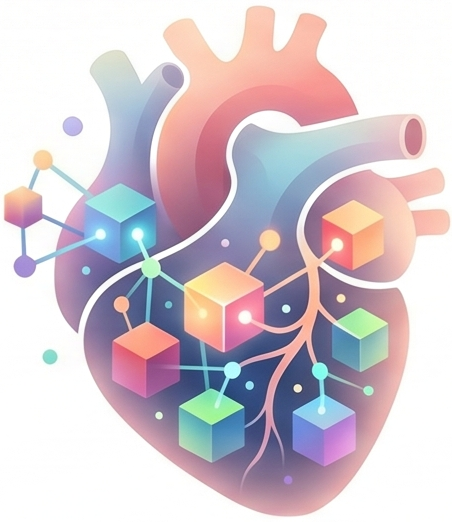
\includegraphics[height=1.5em]{figures/heart-bench-logo.png}}% 请将 logo.png 替换为你的文件名
  \hspace{0.3em} % 控制图标和后面文字之间的空白距离
}

% benchmark comparison table colours & commands
\definecolor{BenchHeaderBg}{RGB}{40, 100, 175}
\definecolor{BenchAltRow}{RGB}{230, 240, 252}
\definecolor{BenchOursRow}{RGB}{195, 240, 205}

\newcommand{\cmark}{\textcolor{green!60!black}{\ding{51}}}
\newcommand{\xmark}{\textcolor{red!70!black}{\ding{55}}}
\newcommand{\pmark}{\textcolor{orange!80!black}{\textbf{\textasciitilde}}}
\newcommand{\bhead}[1]{\textcolor{white}{\textbf{\small #1}}}

\newcommand{\todoc}[2]{{\textcolor{#1}{\textbf{[#2]}}}}
\newcommand{\todo}[1]{\todoblue{#1}} % 默认使用蓝色 todo

\newcommand{\todoblue}[1]{\todoc{blue}{\textbf{#1}}}
\newcommand{\todored}[1]{\todoc{red}{\textbf{#1}}}
\newcommand{\todoorange}[1]{\todoc{orange}{\textbf{#1}}}
\newcommand{\todopurple}[1]{\todoc{pruple}{\textbf{#1}}}

\newcommand{\peng}[1]{\todoblue{peng: #1}}
\newcommand{\zhang}[1]{\todoblue{zhang: #1}}
\newcommand{\shi}[1]{\todoorange{shi: #1}}
\newcommand{\gu}[1]{\todored{gu: #1}}

\newcommand{\feng}[1]{\todopurple{Feng: #1}}


\newcommand{\ourbench}[0]{\textsc{HEART-Bench}\xspace}
\newcommand{\hficon}{%
  \raisebox{-0.2\height}{
\includegraphics[height=1em]{figures/hf-logo.pdf}}%
}

\contribnote{equal}{Equal contribution.}
\contribnote{corr}{\Letter}{Corresponding author.}

% Note. For the workshop paper template, both \title{} and \workshoptitle{} are required, with the former indicating the paper title shown in the title and the latter indicating the workshop title displayed in the footnote. 
\title{\heartbenchicon \ourbench: Do LLM Agents Exhibit Human-like Psychology?}
%\title{MentalAIBench: Evaluating Emotional Intelligence of Large Language Models from Psychology}

% The \author macro works with any number of authors. There are two commands
% used to separate the names and addresses of multiple authors: \And and \AND.
%
% Using \And between authors leaves it to LaTeX to determine where to break the
% lines. Using \AND forces a line break at that point. So, if LaTeX puts 3 of 4
% authors names on the first line, and the last on the second line, try using
% \AND instead of \And before the third author name.

\scaiauthor{1,equal}{Weihan Peng}
\scaiauthor{2,equal}{Chenxu Zhang}
\scaiauthor{3,4}{Qianao Wang}
\scaiauthor{1}{Yuling Shi}
\scaiauthor{1}{Heng Lian}
\scaiauthor{3}{Qihong Mao}
\scaiauthor{5}{Jiahao Pang}
\scaiauthor{5}{Chunliang Feng}
\scaiauthor{3}{Bowen Li}
\scaiauthor{1,corr}{Xiaodong Gu}

\affiliation{1}{Shanghai Jiao Tong University}
\affiliation{2}{Imperial College London}
\affiliation{3}{Quwan Group}
\affiliation{4}{University of Washington}
\affiliation{5}{South China Normal University}

% \author{%
% \textbf{Weihan Peng\textsuperscript{\dag}}$^{1}$,
% \textbf{Chenxu Zhang\textsuperscript{\dag}}$^{2}$,
% \textbf{Qianao Wang}$^{3,4}$,
% \textbf{Yuling Shi}$^{1}$,
% \textbf{Heng Lian}$^{1}$,
% \textbf{Qihong Mao}$^{3}$,\\
% \textbf{Jiahao Pang}$^{5}$,
% \textbf{Chunliang Feng}$^{5}$,
% \textbf{Bowen Li}$^{3}$,
% \textbf{Xiaodong Gu\textsuperscript{{\textrm{\Letter}}}}$^{1}$\\
% $^{1}$Shanghai Jiao Tong University,
% $^{2}$Imperial College London,
% $^{3}$Quwan Group,\\
% $^{4}$University of Washington
% $^{5}$South China Normal University\\
% \\
%   \faGithub\ GitHub: \href{https://github.com/peng-weihan/HEART-BENCH}{https://github.com/peng-weihan/HEART-BENCH}
%   \\
%    \hficon\ Hugging Face: \href{https://huggingface.co/datasets/HEART-BENCH/HEART-BENCH}{https://huggingface.co/datasets/HEART-BENCH/HEART-BENCH}
% % $^{\dag}$Equal contribution
% % $^{*}$Corresponding author
%   % David S.~Hippocampus\thanks{Use footnote for providing further information
%   %   about author (webpage, alternative address)---\emph{not} for acknowledging
%   %   funding agencies.} \\
%   % Department of Computer Science\\
%   % Cranberry-Lemon University\\
%   % Pittsburgh, PA 15213 \\
%   % \texttt{hippo@cs.cranberry-lemon.edu} \\
%   % examples of more authors
%   % \And
%   % Coauthor \\
%   % Affiliation \\
%   % Address \\
%   % \texttt{email} \\
%   % \AND
%   % Coauthor \\
%   % Affiliation \\
%   % Address \\
%   % \texttt{email} \\
%   % \And
%   % Coauthor \\
%   % Affiliation \\
%   % Address \\
%   % \texttt{email} \\
%   % \And
%   % Coauthor \\
%   % Affiliation \\
%   % Address \\
%   % \texttt{email} \\
% }

\begin{document}

% \begin{tikzpicture}[remember picture,overlay]

% \node[anchor=north west] at ([xshift=0.4cm, yshift=-0.4cm]current page.north west) {
%     
\includegraphics[width=1.8cm]{figures/sjtu.pdf}
% };

% \node[anchor=north west] at ([xshift=2.4cm, yshift=-0.4cm]current page.north west) {
%     
\includegraphics[width=1.8cm]{figures/icl.pdf}
% };

% \node[anchor=north west] at ([xshift=4.2cm, yshift=-0.8cm]current page.north west) {
%     
\includegraphics[width=1.8cm]{figures/uw.pdf}
% };

% \node[anchor=north west] at ([xshift=6.2cm, yshift=-0.4cm]current page.north west) {
%     
\includegraphics[width=1.6cm]{figures/scnu.pdf}
% };

% \node[anchor=north east] at ([xshift=-1cm, yshift=-0.8cm]current page.north east) {
%     
\includegraphics[width=2.5cm]{figures/quwan.pdf}    
% };

% \end{tikzpicture}


% {\renewcommand{\thefootnote}{}
% \footnotetext{\textsuperscript{\dag}Equal contribution. {\textrm{\Letter}}\,Corresponding author.}}

\begin{abstract}
While LLM agents have demonstrated remarkable task-oriented abilities such as planning, reasoning, and action, few works have treated them as complete human personalities where emotional dimensions hold equal importance. In this paper, we introduce a novel benchmark to systematically assess whether LLM agents can simulate coherent, human-like psychology. Specifically, our benchmark constructs 11 diverse human characters grounded in orthogonal Big Five personality traits, with each profile deeply integrated with 1,000 structured autobiographical-style episodic memories distributed across theory-grounded developmental life stages. To rigorously evaluate the psychological manifestations of LLMs, we designed a curated suite of 64 decision-making scenarios, guided by the DIAMONDS taxonomy, a psychological framework that characterizes situations along eight dimensions: Duty, Intellect, Adversity, Mating, pOsitivity, Negativity, Deception, and Sociality. By subjecting agents to varying scenarios, the benchmark evaluates whether they can consolidate their innate personality traits and autobiographical memories to make behavioral decisions that are consistent with their specific psychological profiles. After systematic human validation and filtering, we obtained a benchmark consisting of 673 multiple-choice questions (MCQs). We believe this benchmark provides a principled and scalable testbed for studying human-like emotions, personality consistency, and value-consistent behavioural decision-making in LLM-based agents.
\end{abstract}

\metadata[\faGithub]{https://github.com/peng-weihan/HEART-BENCH}
\metadata[\hficon]{https://huggingface.co/datasets/HEART-BENCH/HEART-BENCH}

\maketitle
\section{Introduction}
\label{sec:Introduction}

The rapid advancement of Large Language Models (LLMs) has driven remarkable breakthroughs across numerous domains \cite{anthropic2026claudeopus47,openai2026gpt55,google2026gemini31pro}. However, existing research predominantly concentrates on task-oriented accuracy and conversational reasoning capabilities, rarely treating AI agents as complete human personalities where emotional dimensions hold equal importance. This raises a question: \emph{Do LLM agents exhibit human-like psychological characteristics, such as emotions and value-orientations?} This question might seem far-fetched, yet answering it has profound implications: As LLMs become increasingly integrated into entertainment \cite{chen2024persona,tseng2024two}, companionship \cite{maples2024loneliness,phang2025investigating}, and persona-cloning \cite{wei2025ai, lee2026creating} that simulate individual users, user expectations for these systems have shifted from task-oriented assistance toward persistent, personalized, and psychologically consistent interaction that more closely resembles human-like interaction patterns. When these capabilities are realized and effectively integrated, such systems may begin to exhibit early forms of affective intelligence \cite{marcus2000affective}, enabling more human-like personality consistency and long-term identity coherence. This represents a critical step toward higher-level artificial Emotional Intelligence (EI) \cite{salovey1990emotional}.
% As LLMs become increasingly integrated into entertainment \cite{tseng2024two}, social networking \cite{?}, and emotional companionship \cite{chen2024persona}, user expectations for anthropomorphic AI agents have evolved from merely task assistant to providing long-term emotional companionship. When these capabilities are realized and effectively synergized, AI agents may acquire the foundational prerequisites for more advanced forms of affective intelligence—a critical milestone in the pursuit of higher artificial Emotional Intelligence (EI) \cite{?}.

Despite these evolving expectations, the current landscape of evaluation frameworks remains heavily constrained. Existing benchmarks primarily measure short- and long-term conversational context, explicit reasoning, memory recall, and end-to-end question-answering accuracy. While these efforts establish a foundational assessment framework for cognitive capabilities, merely advancing "conversation" and "memory" is insufficient. In the domain of evaluating the human-like psychology of AI agents, standardized evaluation frameworks are still in their early stages of development.

To bridge this gap, we introduce \ourbench (\textbf{H}uman-like \textbf{E}motion and \textbf{A}gent \textbf{R}eaction \textbf{T}est), a novel benchmark specifically designed to quantify the human-like psychology of AI Agents. Our benchmark aims to facilitate the development of ``high-EI'' AI agents and significantly enhance the user experience in human-AI interactions.
Specifically, our benchmark simulates 11 diverse human characters. Each character is grounded in a foundational five-dimensional personality framework (e.g., the Big Five personality traits) and is intricately associated with 1,000 episodes of autobiographical memory~\cite{singer1995seeing} spanning distinct life stages. To rigorously evaluate the psychological manifestations of LLMs, we designed 64 evaluation scenarios woven into these key life milestones. Each (character, scenario) tuple is annotated by psychology experts with the expected behavioural decision, and the resulting annotations are assembled into multiple-choice questions (MCQs) in which the target character's response is the ground truth and other characters' responses to the same scenario serve as distractors. After systematic expert validation and filtering, HEART-BENCH contains 673 multiple-choice evaluation instances in total. During the evaluation process, the model is exposed to scenario triggers that elicit emotional responses, requiring the LLM to reason over the character’s basic publicly available settings and prior memories, and to select appropriate behavioral decisions.
% The rapid advancement of Large Language Models (LLMs) has driven remarkable breakthroughs across numerous domains. However, existing research predominantly concentrates on task-oriented accuracy and conversational reasoning capabilities, rarely treating AI agents as complete human personalities where emotional dimensions hold equal importance. This raises an open question:\textcolor{blue}{ \emph{Do LLM agents exhibit human-like psychological characteristics, such as emotions and inherent values?}} This question sounds highly forward-looking, yet answering it has profound implications: As LLMs become increasingly integrated into entertainment, social networking, and emotional companionship, user expectations for anthropomorphic AI agents have evolved from simply "conversing like a human" to providing "long-term, memory-grounded emotional companionship." When these capabilities are fully realized and effectively synergized, AI agents will possess the foundational prerequisites for generating "human-like consciousness"—a critical milestone in the pursuit of higher artificial Emotional Intelligence (EI).

% Despite these evolving expectations, the current landscape of evaluation frameworks remains heavily constrained. Existing benchmarks primarily measure short- and long-term conversational context, explicit reasoning, memory recall, and end-to-end question-answering accuracy. While these efforts establish a foundational assessment framework for cognitive capabilities, merely advancing "conversation" and "memory" is insufficient. A pervasive lack of genuine "human touch" and empathy remains a significant bottleneck during long-term human-AI interactions. In the specific domain of evaluating the human-like psychology of AI agents, there is currently a complete void of standardized evaluation frameworks.

% To bridge this gap, we introduce \ourbench, a novel benchmark specifically designed to quantify the "human-like psychology of AI Agents." Our benchmark aims to facilitate the development of ``high-EI'' AI agents and significantly enhance the user experience in human-AI interactions.
% Specifically, our benchmark simulates 20 diverse human characters. Each character is grounded in a foundational five-dimensional personality framework (e.g., the Big Five personality traits) and is intricately associated with 1,000 memory episodes spanning distinct life stages. To rigorously evaluate the psychological manifestations of LLMs, we designed 50 evaluation scenarios woven into these key life milestones. During the evaluation process, the models are subjected to emotion-eliciting queries, requiring the LLM to reason over the characters' prior memory up to that age and infer the appropriate behavioral decision. 

%Our benchmark involves XXXX characters and XXXX scenarios, each is structured, psychologically informed. \gu{Give an overall description of the benchmark}. We constructs each \gu{Add description about characters} scenario using a hierarchical schema that explicitly models developmental stages, contextual environments, emotional dynamics, and decision-critical events. In particular, we incorporate psychological dimensions inspired by the DIAMONDS framework\cite{} in psychology to characterize situational structure and intensity, enabling fine-grained control over cognitive and emotional demands.

%Each scenario simulates a realistic interaction loop in which an agent must interpret contextual information, integrate long-term memory, and make value-consistent decisions under uncertainty. This design allows us to move beyond surface-level recall tasks toward evaluating whether agents can maintain coherent identity, adapt to evolving contexts, and exhibit consistent value-oriented behavior over time.


We benchmark twelve frontier LLMs---spanning the GPT, Claude, Gemini, DeepSeek, and Qwen families—under three interactive settings (Naive-RAG~\cite{lewis2020retrieval}, Mem0~\cite{chhikara2025mem0}, and PersonaDB~\cite{sun2025persona}), together with a vanilla LLM baseline. Across all settings, even the strongest model (Gemini-3.1-Pro) achieves at most
63.3\% accuracy, while most models remain below 40\%, highlighting a clear performance bottleneck. We believe this benchmark provides a principled and scalable testbed for studying human-like emotion, personality consistency, and value alignment in LLM-based agents.

We summarize our contributions as follows:
\begin{itemize}[leftmargin=2em]
    \item We propose \ourbench{}, a high-quality benchmark comprising 11 validated characters and 64 challenging scenarios, accompanied by expert annotations and 673 multiple-choice questions.
    \item We provide a systematic evaluation framework to evaluate LLMs' human-like psychology. 
    \item We evaluate multiple LLMs in varying agentic settings. Results show that the ability of LLMs to exhibit human-like psychology remains limited.
\end{itemize}


% \begin{table}[t]
% \centering
% \small
% \caption{Comparison of \ourbench with related benchmarks across key dimensions.
% \cmark~yes;~~\xmark~no;~~\pmark~partial.
% \emph{Lifespan coverage}: explicit multi-stage developmental design (e.g., childhood, adolescence, adulthood) grounded in developmental psychology—multi-session dialogue time spans do not qualify.}
% \label{tab:benchmark_comparison}
% \begin{tabular}{lccccc}
% \toprule
% \textbf{Benchmark} &
% \textbf{\makecell{Big-Five\\grounded}} &
% \textbf{\makecell{Lifespan\\coverage}} &
% \textbf{\makecell{Episodic\\memory}} &
% \textbf{\makecell{Scenario\\eval.}} &
% \textbf{\makecell{Expert\\annot.}} \\
\begin{table}[t]
\centering
\footnotesize
\caption{Comparison of \ourbench with related benchmarks across six dimensions (see Appendix~\ref{app:benchmark_dims} for dimension definitions).
\cmark~yes;~~\xmark~no;~~\pmark~partial.}
\label{tab:benchmark_comparison}
\resizebox{\textwidth}{!}{
\begin{tabular}{lcccccc}
\toprule
\textbf{Benchmark} &
\textbf{Big-Five grounded} &
\textbf{Lifespan coverage} &
\textbf{Episodic memory} &
\textbf{Scenario eval.} &
\textbf{Expert annot.} &
\textbf{\makecell{Trait-driven\\decision}} \\
\midrule
%KnowMeBench~\cite{wu2026knowme}          & \xmark & \pmark & \pmark & \pmark & \cmark & \xmark \\
\rowcolor{BenchAltRow}
CharacterEval~\cite{tu2024charactereval} & \xmark & \xmark & \xmark & \cmark & \pmark & \xmark \\
PersonaHub~\cite{ge2024scaling}       & \xmark & \xmark & \xmark & \cmark & \xmark & \xmark \\
\rowcolor{BenchAltRow}
LoCoMo~\cite{maharana2024evaluating}     & \xmark & \xmark & \cmark & \cmark & \xmark & \xmark \\
%LongMemEval~\cite{wu2024longmemeval}     & \xmark & \xmark & \cmark & \cmark & \xmark & \xmark \\
CloneMem~\cite{hu2026clonemem}           & \cmark & \pmark & \cmark & \xmark & \xmark & \xmark \\
\rowcolor{BenchAltRow}
%RealMem~\cite{bian2026realmem}           & \xmark & \pmark & \cmark & \cmark & \xmark & \xmark \\
PersonaLens~\cite{zhao2025personalens}   & \xmark & \xmark & \pmark & \cmark & \pmark & \xmark \\
PersonaMem~\cite{jiang2025personamem}    & \xmark & \xmark & \pmark & \cmark & \xmark & \xmark \\
\midrule
\rowcolor{BenchOursRow}
\textbf{\ourbench}       & \cmark & \cmark & \cmark & \cmark & \cmark & \cmark \\
\bottomrule
\end{tabular}
}
\vspace{-10pt}
\end{table}


\section{Related Work}

%\subsection{Role-Playing and Persona-Aware Agent Systems}
% \subsection{Psychology-Grounded Benchmarks}

%\subsection{Persona-Aware Agent Systems}
%\shi{A bit too long now}
%\peng{shrink after later}
\subsection{Personality Modeling in LLM Agents}
The Big Five (OCEAN) framework~\cite{mccrae1992introduction} is the dominant operationalization of stable individual differences in personality psychology, with well-established predictive validity across cultures~\cite{mccrae1997personality} and the lifespan~\cite{roberts2007power}. A key theoretical insight is that personality is not a fixed behavioral template but a dynamic disposition. Fleeson's whole-trait theory~\cite{fleeson2001toward} frames each trait as a density distribution of behavioral states that shifts with situational demands, while Conway \& Pleydell-Pearce~\cite{conway2000construction} show that autobiographical memories are organized hierarchically around self-relevant goals, binding identity to lived experience. Young's schema therapy~\cite{young2006schema} further documents how early maladaptive schemas—crystallized at developmentally critical periods—propagate their influence on emotional reactivity and decision-making throughout adulthood. These core insights from personality and clinical psychology remain largely unincorporated in existing LLM persona work.



Current LLM persona systems fall into two broad lines. The first encodes personality as a static profile injected at inference time: Character-LLM~\cite{shao2023character} and PersonaLLM~\cite{jiang2024personallm} condition generation on fixed role descriptions or trait vectors, PersonaAgent~\cite{zhang2025personaagent} extends this with Big Five-conditioned behavioral adaptation, and RGMem~\cite{tian2025rgmem} further modulates expression based on contextual relationships. The second line prioritizes memory infrastructure—MemGPT~\cite{packer2023memgpt}, HippoRAG~\cite{gutierrez2024hipporag}, Mem0~\cite{chhikara2025mem0}, and A-MEM~\cite{xu2025mem} provide scalable long-term retrieval substrates. While these offer necessary engineering foundations, neither line addresses the core psychological question: how does a character's trait profile shape which experiences are encoded, how mood-congruent processes~\cite{bower1981} color their emotional valence, and how this accumulated life history produces coherent, personality-driven responses in novel situations.


\subsection{Benchmarks for Psychology-Grounded Agent Evaluation}
\textbf{Psychometric evaluation of LLMs.}
A growing body of work examines whether LLMs can exhibit human-like personality profiles. Prompted LLMs can simulate Big Five questionnaire responses with reasonable reliability~\cite{serapio2023personality}, while subsequent studies apply MBTI or Big Five scales to characterize model behavior. However, these approaches use psychometric instruments as \emph{input stimuli}—probing how models respond to trait questionnaires—rather than as \emph{evaluation criteria} for whether behavioral decisions in rich, naturalistic contexts are consistent with a given personality profile. They also treat personality as a static, context-free attribute, overlooking its developmental dimension: McAdams's narrative identity theory~\cite{mcadams2001psychology} establishes that personality is expressed through the life story an individual constructs over time, and Pasupathi et al.~\cite{pasupathi2007developing} show that self-relevant narration actively shapes trait expression across life stages. Psychometric snapshots capture neither of these longitudinal dynamics.

\textbf{Persona and memory benchmarks.}
Conversational persona benchmarks typically supply a personality description via system prompt and then test factual or stylistic consistency. Long-horizon benchmarks such as LoCoMo~\cite{maharana2024evaluating} and LongMemEval~\cite{wu2024longmemeval} extend this to multi-session dialogues, but personality remains a static backdrop: the focus is on what agents recall, not on how trait profiles shape the encoding and emotional interpretation of experience. More recent work incorporates richer sources—CloneMem~\cite{hu2026clonemem} uses heterogeneous data (diaries, social media) grounded in Big Five personas; RealMem~\cite{bian2026realmem} tracks goal consistency across project-oriented sessions; KnowMeBench~\cite{wu2026knowme} probes preference inference from personal narratives. These are meaningful steps, yet their primary evaluation targets remain closer to recall, preference inference, or goal-consistency tracking than to trait-grounded behavioural decision-making under controlled psychological scenarios. \ourbench instead conditions every decision on a character's Big Five profile and 1,000 trait-shaped autobiographical memories, and evaluates behavioural choice under controlled DIAMONDS-structured scenarios~\cite{rauthmann2014diamonds}, shifting the evaluation target from recall and preference inference to trait-grounded behavioural decision-making.

\textbf{Data substrates and evaluation depth.}
A shared limitation is the quality of underlying data. Most benchmarks rely on synthetic chat logs or sandboxed interactions, which lack the sensory concreteness and introspective density that characterize genuine autobiographical memory~\cite{rubin2006basic}. Such shallow substrates constrain what evaluation can detect: without episodic content structured around perceptual, affective, and somatic dimensions, benchmarks cannot distinguish agents that reason from stable psychological principles from those that merely pattern-match on surface cues. The absence of lifespan-grounded coverage further means that no existing benchmark can assess whether personality remains coherent across developmental transitions—the longitudinal consistency that McAdams~\cite{mcadams2001psychology} identifies as the hallmark of integrated personal identity. \ourbench addresses both gaps by generating each memory under Rubin's Basic Systems~\cite{rubin2006basic} Model with integrated sensory, dialogic, introspective, somatic, and aftermath content, and distributing the 11,000-memory corpus across eight Erikson–Levinson developmental stages~\cite{erikson1963childhood,levinson1978seasons} from ages 6 to 50.
% \gu{Compared to these related works, what are the strengths and differences of ours?}.
Table~\ref{tab:benchmark_comparison} summarizes how \ourbench differs from representative prior benchmarks across six dimensions central to psychology-grounded evaluation.

\begin{figure}[t]
    \centering
    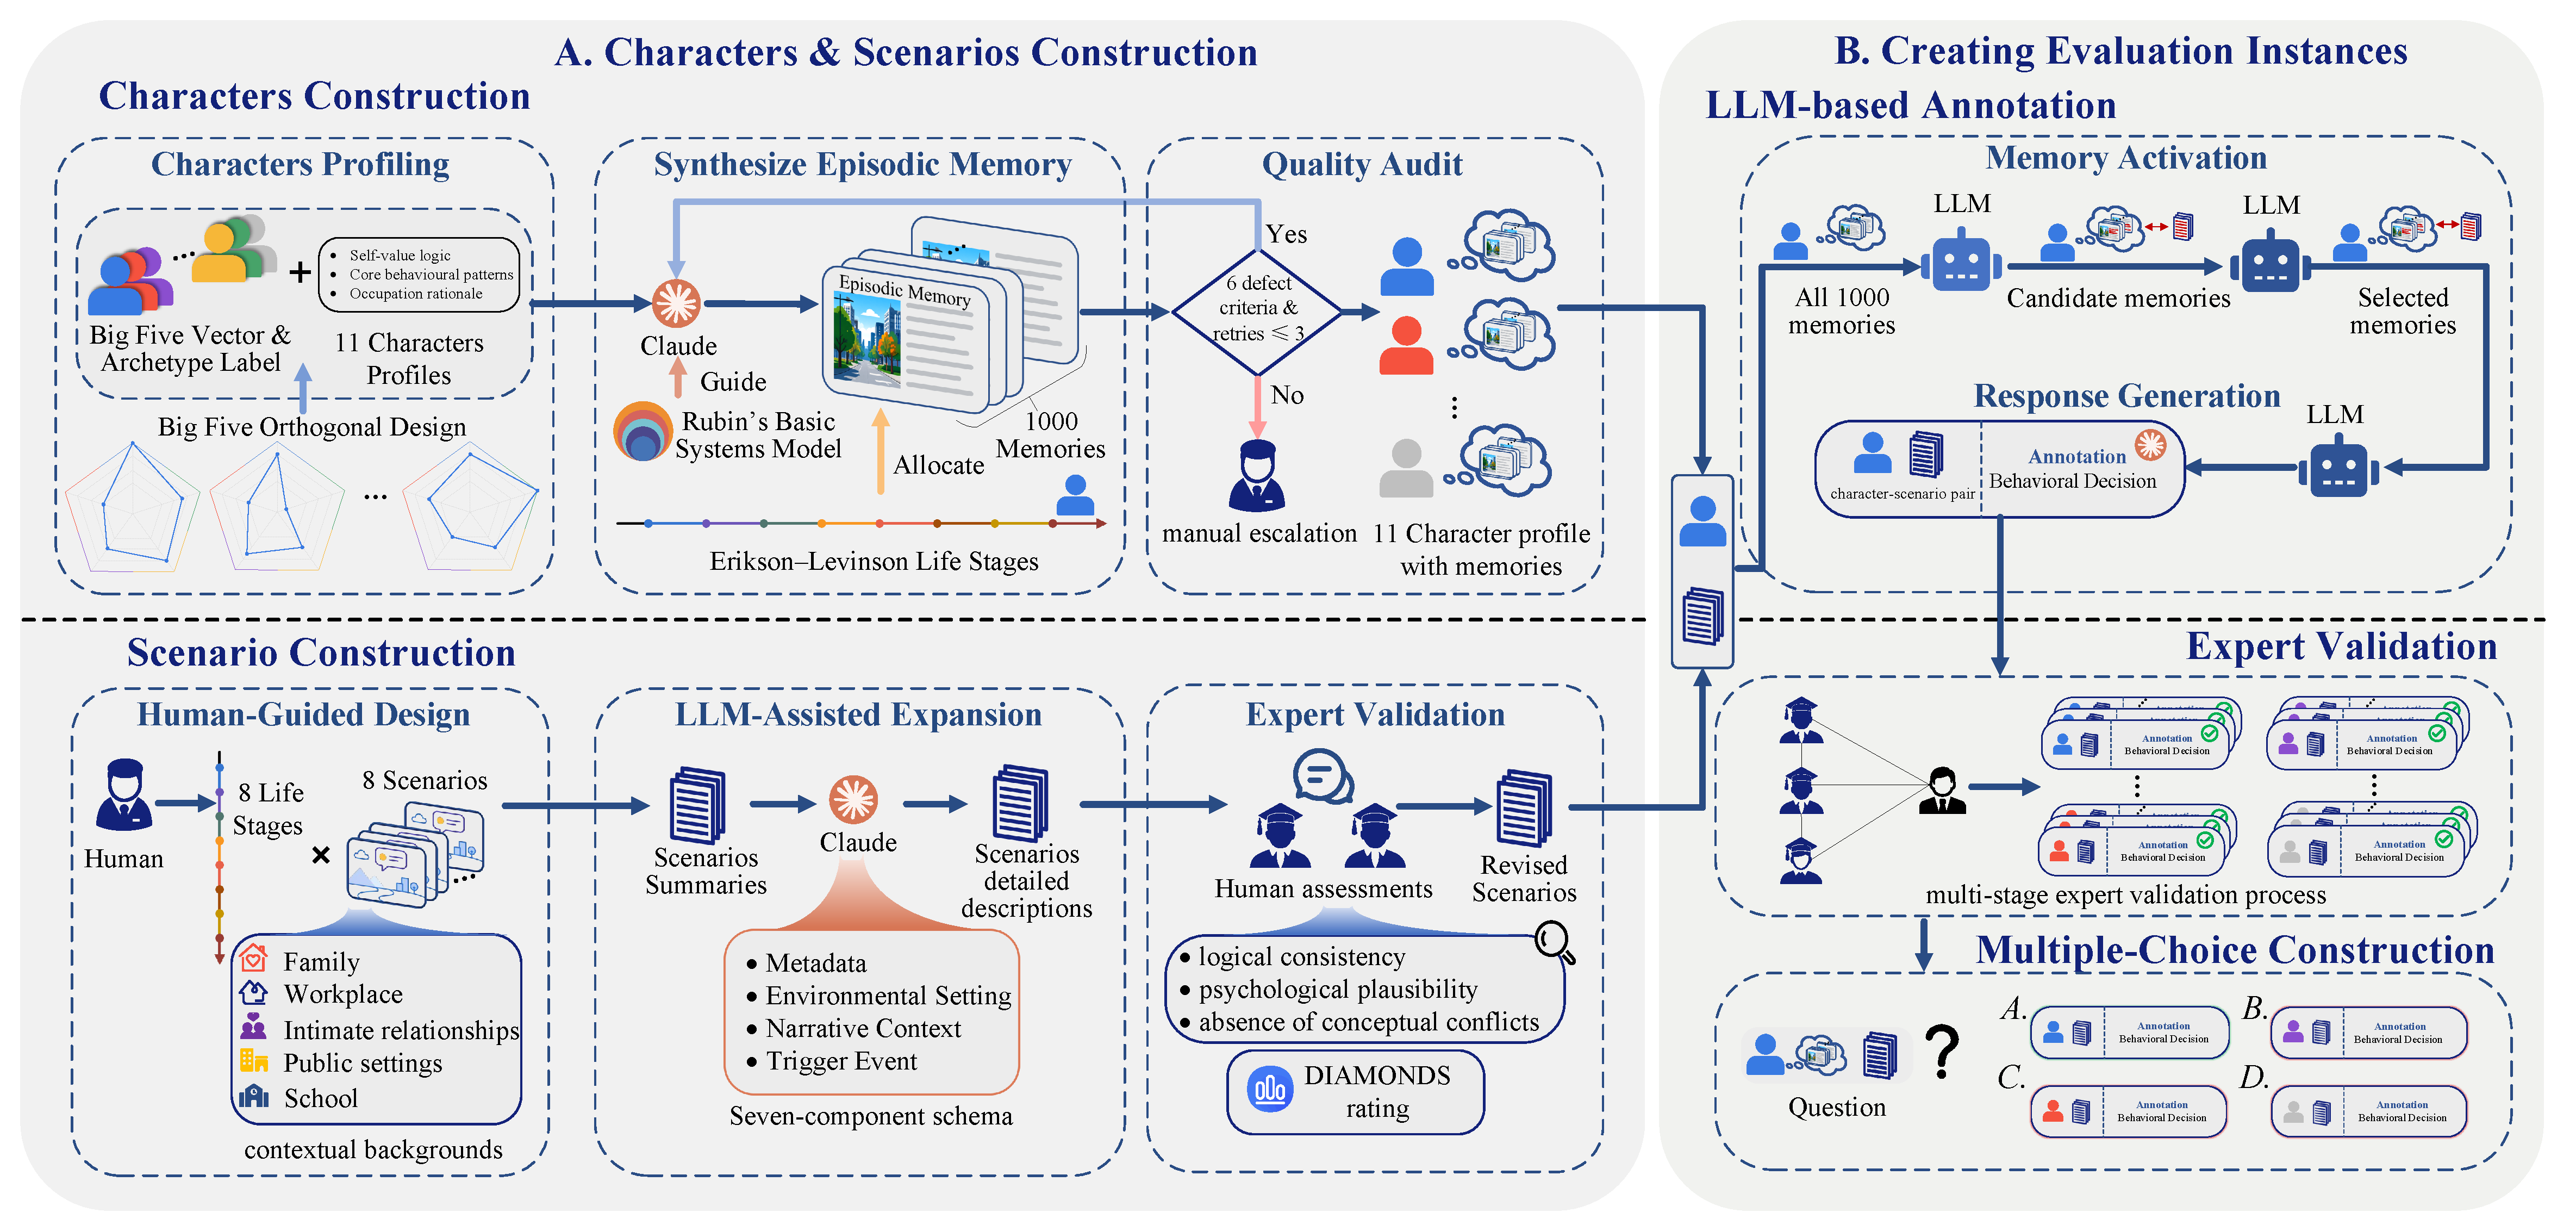
\includegraphics[width=1\linewidth]{figures/pipeline.pdf}
    \caption{The pipeline has four stages: character construction for generating stable personas and scenario construction to elicit behavioral differences. This is followed by ground-truth annotation to define expected responses, and finally conversion into MCQ format for model evaluation.}
    \label{fig:pipeline}
    \vspace{-10pt}
\end{figure}

\section{\ourbench}
\subsection{Overview}

Figure~\ref{fig:pipeline} illustrates the full pipeline of \ourbench. The benchmark comprises two components---an 11-persona \emph{character set} grounded in the Big Five~\cite{mccrae1992introduction} and Schwartz's value theory~\cite{schwartz1992universals}, with each character equipped with $1{,}000$ long-horizon memories, and a \emph{scenario suite} of 64 character-agnostic situations that span the eight DIAMONDS~\cite{rauthmann2014diamonds} dimensions---\emph{Duty}, \emph{Intellect}, \emph{Adversity}, \emph{Mating}, p\emph{O}sitivity, \emph{N}egativity, \emph{D}eception, and \emph{S}ociality---across the lifespan. Each (character, scenario) tuple is annotated and validated by experts with the expected behavioural decision, and the resulting annotations are assembled into multiple-choice questions in which the target character's response is the ground truth and other characters' responses to the same scenario serve as distractors. After systematic human validation and filtering, \ourbench contains $673$ multiple-choice evaluation instances in total.

\begin{wraptable}{r}{0.42\linewidth}
\vspace{-12pt}
\centering
\captionof{table}{Statistics of \ourbench.}
\label{tab:dataset_overview}
\small
\begin{tabular}{lc}
\toprule
\textbf{Statistic} & \textbf{Value} \\
\midrule
Characters           & 11 \\
Memories / character & 1{,}000 \\
Length / character   & $\sim$1.4M tokens \\
Life stages          & 8 (ages 6--50) \\
Scenarios            & 64 \\
MCQs                 & 673 \\
\bottomrule
\end{tabular}
\vspace{-10pt}
\end{wraptable}

\subsection{Characters Construction}
\label{sec:character}

% ---- Formal Notation ----
To construct AI characters capable of demonstrating genuine psychological depth, we define a character as a psychologically grounded entity: \(c=(\mathbf{p}, \{m_i\}_{i=1}^{T})\). Here,
$\mathbf{p} = (O, C, E, A, N) \in [0,1]^5$ denotes a Big Five trait vector, and \(\{m_i\}_{i=1}^{T})\) represents a lifelong sequence of autobiographical memories~\cite{singer1995seeing}. 
% An episodic memory \(m_i\) is a structured tuple
% \begin{equation}
%   m_i \;=\; \bigl\langle\,\tau,\; x_{\mathrm{ctx}},\; x_{\mathrm{sum}},\; x_{\mathrm{full}},\;
%           \mathbf{r},\; \psi\,\bigr\rangle,
%   \label{eq:memory}
% \end{equation}
% with $\tau \in [6, 50]$ the age at encoding, $x_{\mathrm{ctx}}$ a compact situational setting, $x_{\mathrm{sum}}$ a one-sentence gist, $x_{\mathrm{full}}$ the full first-person narrative, $\mathbf{r}$ retrieval-index fields (triggers and relevance tags), and $\psi$ psychological annotations (psych conclusion, behaviour policy, emotion signature). The complete ten-field schema is detailed in Appendix~\ref{app:stats}.
Rather than relying on superficial prompts, we engineer these characters through a rigorous, three-stage developmental pipeline.

% ---- Stage A ----
%\paragraph{Stage 1: Psychological Blueprinting.}
\textbf{Stage 1: Character Profiling.}
The foundation of our benchmark requires clean attribution: if an AI agent behaves a certain way, we must be able to trace it back to a specific psychological trait without confounding variables. Unlike prior persona-based benchmarks that inject loosely defined personality descriptions at inference time~\citep{shao2023character,jiang2024personallm}, we adopt a principled Big Five orthogonal design~\citep{mccrae1992introduction} in which each character is anchored to a single dominant trait at an extreme value, enabling controlled, interpretable comparisons across characters.
Concretely, we isolate each of the five OCEAN dimensions by creating one high-extreme ($p = 0.95$) and one low-extreme ($p = 0.10$) profile per trait, alongside one neutral baseline ($p = 0.50$ on all dimensions). This yields $|\mathcal{C}| = 11$ archetypes (summarized in Table~\ref{tab:characters}) with a strict pairwise $\ell_\infty$ separation: $\forall\, i \neq j,\ \|\mathbf{p}_i - \mathbf{p}_j\|_\infty \geq 0.45$.
This separation ensures that behavioural differences between any two characters are primarily attributable to a single dominant trait, substantially reducing the risk of confounded comparisons.

To maintain ecological validity, each character is assigned an occupation congruent with their dominant trait (e.g., a high-Neuroticism freelance creator versus a low-Neuroticism community general practitioner). Furthermore, each profile encodes a distinct "self-value logic" and eight core behavioral patterns, which act as strict constraints for downstream memory generation (see Appendix~\ref{app:stage_a} for full character specifications and Appendix~\ref{app:prompt_character} for the generation prompt).

% ---- Stage B ----
\textbf{Stage 2: Synthesizing Autobiographical Memories.}
While the Big Five trait vectors provide the static skeleton of a character's profile, genuine human psychology is dynamically shaped by cumulative life experiences. In narrative psychology, \textbf{autobiographical memories}~\cite{singer1995seeing} serve as the bedrock of identity—they dictate how an individual interprets the present, evaluates threats, and makes future decisions. To transform our AI characters into agents with true psychological depth, we populate their lifespans with 1,000 episodic memories, each structured around Rubin's Basic Systems Model~\cite{rubin2006basic} (Figure~\ref{fig:rubin}). Rather than a sterile log of actions, every narrative organically weaves together five perceptual-cognitive dimensions: \textit{sensory detail}, \textit{dialogue reconstruction}, \textit{inner monologue}, \textit{somatic response}, and \textit{aftermath} (full definitions in Appendix~\ref{app:stage_c}).


\begin{wrapfigure}{r}{0.42\linewidth}
\vspace{-10pt}
\centering
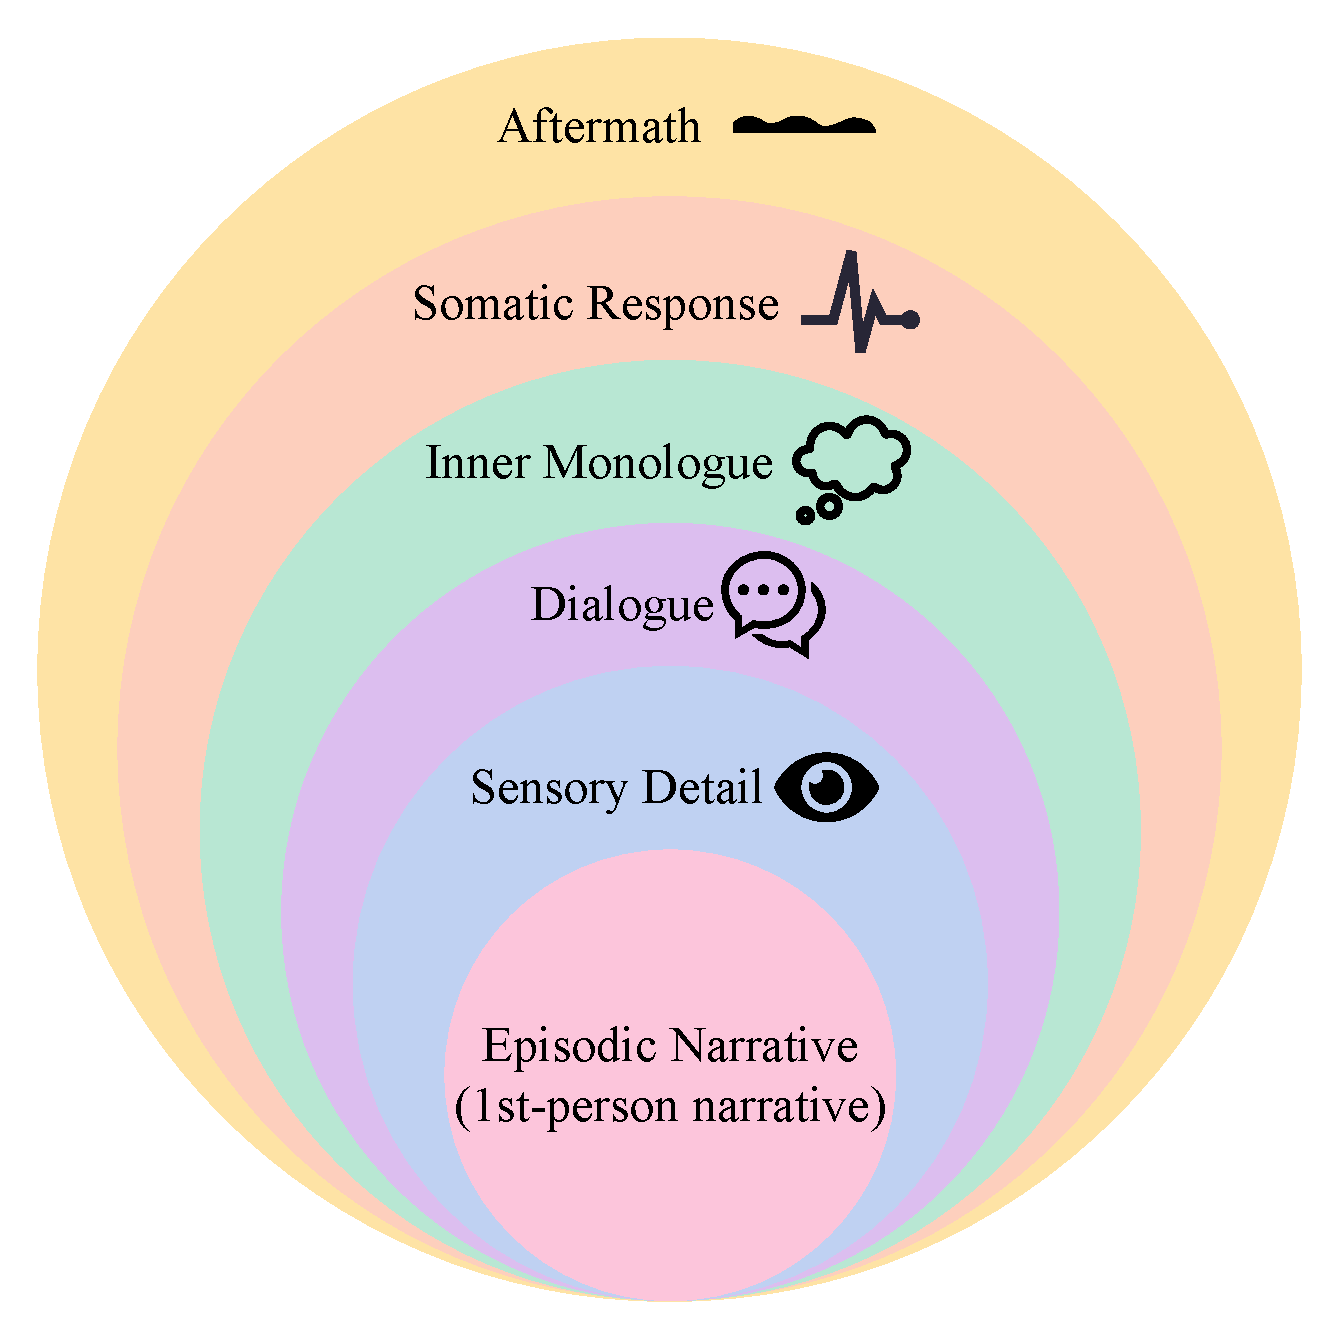
\includegraphics[width=0.85\linewidth]{figures/rubin_model.pdf}
\caption{Rubin's Basic Systems Model~\cite{rubin2006basic} as applied to Episodic Narrative
  generation. Each narrative organically integrates all five dimensions;
  their presence is verified in the Quality Audit stage (Appendix~\ref{app:stage_d}).}
\label{fig:rubin}
\vspace{-10pt}
\end{wrapfigure}


To ground memories in age-appropriate experiences, we map the character's lifespan onto eight developmental macro-stages $\mathcal{S} = \{s_1, \ldots, s_8\}$ by integrating Erikson's psychosocial stages~\cite{erikson1963childhood} (ages 6--18) with Levinson's adult seasons~\cite{levinson1986conception,levinson1978seasons} (ages 18--50; see Appendix~\ref{app:stats}). Memory quota is then distributed across $T = 45$ one-year age bins via a salience weight $w_t$, namely $q_t = \lfloor d \cdot w_t / \sum_j w_j \rfloor$, where $w_t$ is elevated at critical transitions (Adolescence, Early Adult Transition, Age-30 Re-appraisal) and decreases toward midlife~\cite{conway2000construction, young2006schema, singer1995seeing}, yielding a naturally dense, human-like memory distribution (Table~\ref{tab:stage_dist}).

% \begin{table}[h]
% \centering
% \caption{Life-stage schema integrating Erikson~\cite{erikson1963} and Levinson~\cite{levinson1978,levinson1986}.}
% \label{tab:stages}
% \setlength{\tabcolsep}{5pt}
% \begin{tabular}{llll}
% \toprule
% \textbf{Stage} & \textbf{Age} & \textbf{Source} & \textbf{Core task} \\
% \midrule
% School age            & 6--12  & Erikson S4   & Industry vs.\ Inferiority \\
% Adolescence           & 12--18 & Erikson S5   & Identity vs.\ Role Confusion \\
% Early adult trans.\   & 18--22 & Levinson     & Leaving family; world entry \\
% Entering adult world  & 22--28 & Levinson     & Career; intimate relations \\
% Age-30 transition     & 28--33 & Levinson     & Life-structure re-appraisal \\
% Settling down         & 33--40 & Levinson     & Consolidation; mentoring \\
% Midlife transition    & 40--45 & Levinson     & Finitude; identity crisis \\
% Entering midlife      & 45--50 & Levinson+E7  & Generativity; legacy \\
% \bottomrule
% \end{tabular}
% \end{table}

All memories are generated using Claude Sonnet 4.6, with the system prompt injecting $\mathbf{p}_i$, the life-stage context, and diversity constraints across five scenario domains (workplace, interpersonal, health, creative, daily life). Full generation details are in Appendix~\ref{app:stage_c}; the complete system prompt is in Appendix~\ref{app:prompt_memory}.

\textbf{Stage 3: Quality Audit}
Large-scale LLM generation inevitably introduces semantic drift and logical contradictions that rigid formatting validators cannot detect. To guarantee the high fidelity of the memory corpus, we implement a rigorous heuristic auditing framework. Each generated memory is evaluated against six automated defect criteria (details in Appendix~\ref{app:stage_d}). A memory $m$ successfully passes the audit if and only if it violates zero criteria.
% The three primary failure modes we filter for are:
% \textit{perspective drift}—violating the first-person narrative constraint; \textit{duplication}—Near-duplicate episodic generation within the same developmental age window. This is detected using a cosine similarity threshold of $> 0.85$ over TF-IDF vector representations of the narratives; and \textit{age-context mismatch} (e.g., adult-domain vocabulary or themes in memory assigned to childhood stages $\leq 12$).
Memories that fail the audit enter a targeted, closed-loop repair mechanism. %To maintain efficiency and preserve valid context, the system does not regenerate the entire episode; instead, only the specifically defective field is reprompted with an issue-targeted corrective instruction. The pipeline allows up to three autonomous repair attempts per memory before flagging it for manual escalation.
Once fully validated, the memories undergo final integration. They are deduplicated by \texttt{id}, sorted chronologically by age ($\tau$), and compiled into a continuous, 1,000-entry timeline per character. Finally, to prevent demographic confounding variables from skewing downstream LLM evaluations, we sanitize the dataset by replacing all specific character identifiers with gender-neutral labels (e.g., \textit{Role A})~\citep{sun2019mitigating}. The complete schema specification and final corpus statistics are detailed in Appendix~\ref{app:stats}.

\subsection{Scenarios Construction}
\label{sec:scenario}

%We construct a set of scenarios to evaluate whether LLMs can exhibit human-like, persona-consistent behavior under diverse contexts. 
A scenario serves as a structured psychological situation that triggers the AI agent to make a behavioural decision (see Appendix~\ref{app:ExampleofScenario} for a complete example). 
% ---- Formal Notation ----
Formally, a scenario is defined as a tuple
  \(
  s = \bigl\langle\,
    m,\;
    \mathcal{C}_{\mathrm{env}},\; \mathcal{C}_{\mathrm{narrative}},\; e_{\mathrm{trigger}}
  \,\bigr\rangle,
  \)
where $m$ is the developmental and semantic metadata bundling identifiers, scenario name, category, target life stage, age range ($\tau \in [6,50]$), agent description, and intensity level; $\mathcal{C}_{\mathrm{env}}$ describes the environmental context (e.g., location, time, and atmosphere); $\mathcal{C}_{\mathrm{narrative}}$ specifies the narrative background; and $e_{\mathrm{trigger}}$ represents the decision-triggering event that forces the character to make a behavioral decision. Crucially, all scenarios are character-agnostic, written as universal situational descriptions that apply uniformly across the entire character set. This design isolates the agent's internal personality as the sole independent variable, enabling controlled, fair cross-persona comparisons of behavioral responses under identical external stimuli. Note that, despite this character-agnostic design, a small number of character--scenario pairs remain inherently incompatible (e.g., a romantic-partner scenario assigned to a character who is not in a romantic relationship); we explicitly disable such pairs during instance assembly.

\textbf{Stage 1: Human-Guided Blueprinting.} 
To ensure structural diversity, clinical experts manually draft the foundational summaries for all scenarios, utilizing the DIAMONDS~\cite{rauthmann2014diamonds} framework to systematically map out the psychological situation space. We design exactly 8 scenarios per developmental life stage, yielding 64 scenarios across the eight stages in total. These summaries span a highly diverse set of socio-environmental contexts—including family dynamics, school and academic pressures, workplace politics, intimate relationships, and public spaces. Each summary establishes the core situational tension and psychological stakes while strictly maintaining the character-agnostic constraint.

\textbf{Stage 2: LLM-Assisted Expansion.}
We leverage Claude Opus 4.6~\cite{anthropic2026opus46} to expand the expert-drafted summaries into fully realized, high-fidelity scenarios based on a four-component schema (metadata, environmental setting, narrative context, trigger event), enforcing structural consistency across developmental metadata, psychological grounding, and environmental context. The full schema and a complete worked example are given in Appendix~\ref{app:scenario_schema}.

% For example, a human-designed summary for adolescence intellectual challenge becomes a detailed scenario titled "The Classroom Dissent," where a 15-year-old student discovers contradictions between their teacher's historical account and recent academic research they read independently. The scenario specifies the classroom setting ("quiet, dull, slightly oppressive atmosphere"), provides rich narrative context about the authority dynamics, and culminates in the teacher directly asking the student to share their thoughts, requiring a decision on whether to challenge authority with evidence-based disagreement (see Appendix~\ref{app:ExampleofScenario}).
\textbf{Stage 3: Expert Validation.} The generated scenarios are validated by two doctoral-level psychology researchers along two complementary lenses: the DIAMONDS~\cite{rauthmann2014diamonds} taxonomy verifies that each of its eight situational characteristics is exercised across both ends of its intensity range, and Schwartz's value circumplex~\cite{schwartz1992universals} verifies that the central tensions align with theoretically opposing value pairs on the circumplex. The resulting rating distribution and value-conflict spectrum confirm a broad, non-degenerate engagement of the psychological situation space (validation protocol and full coverage distributions in Appendix~\ref{app:scenario_validation}).

\subsection{Creating Evaluation Instances}
\label{sec:CreatingEvaluationInstances}
\begin{figure}[t]
\vspace{-10pt}
\centering
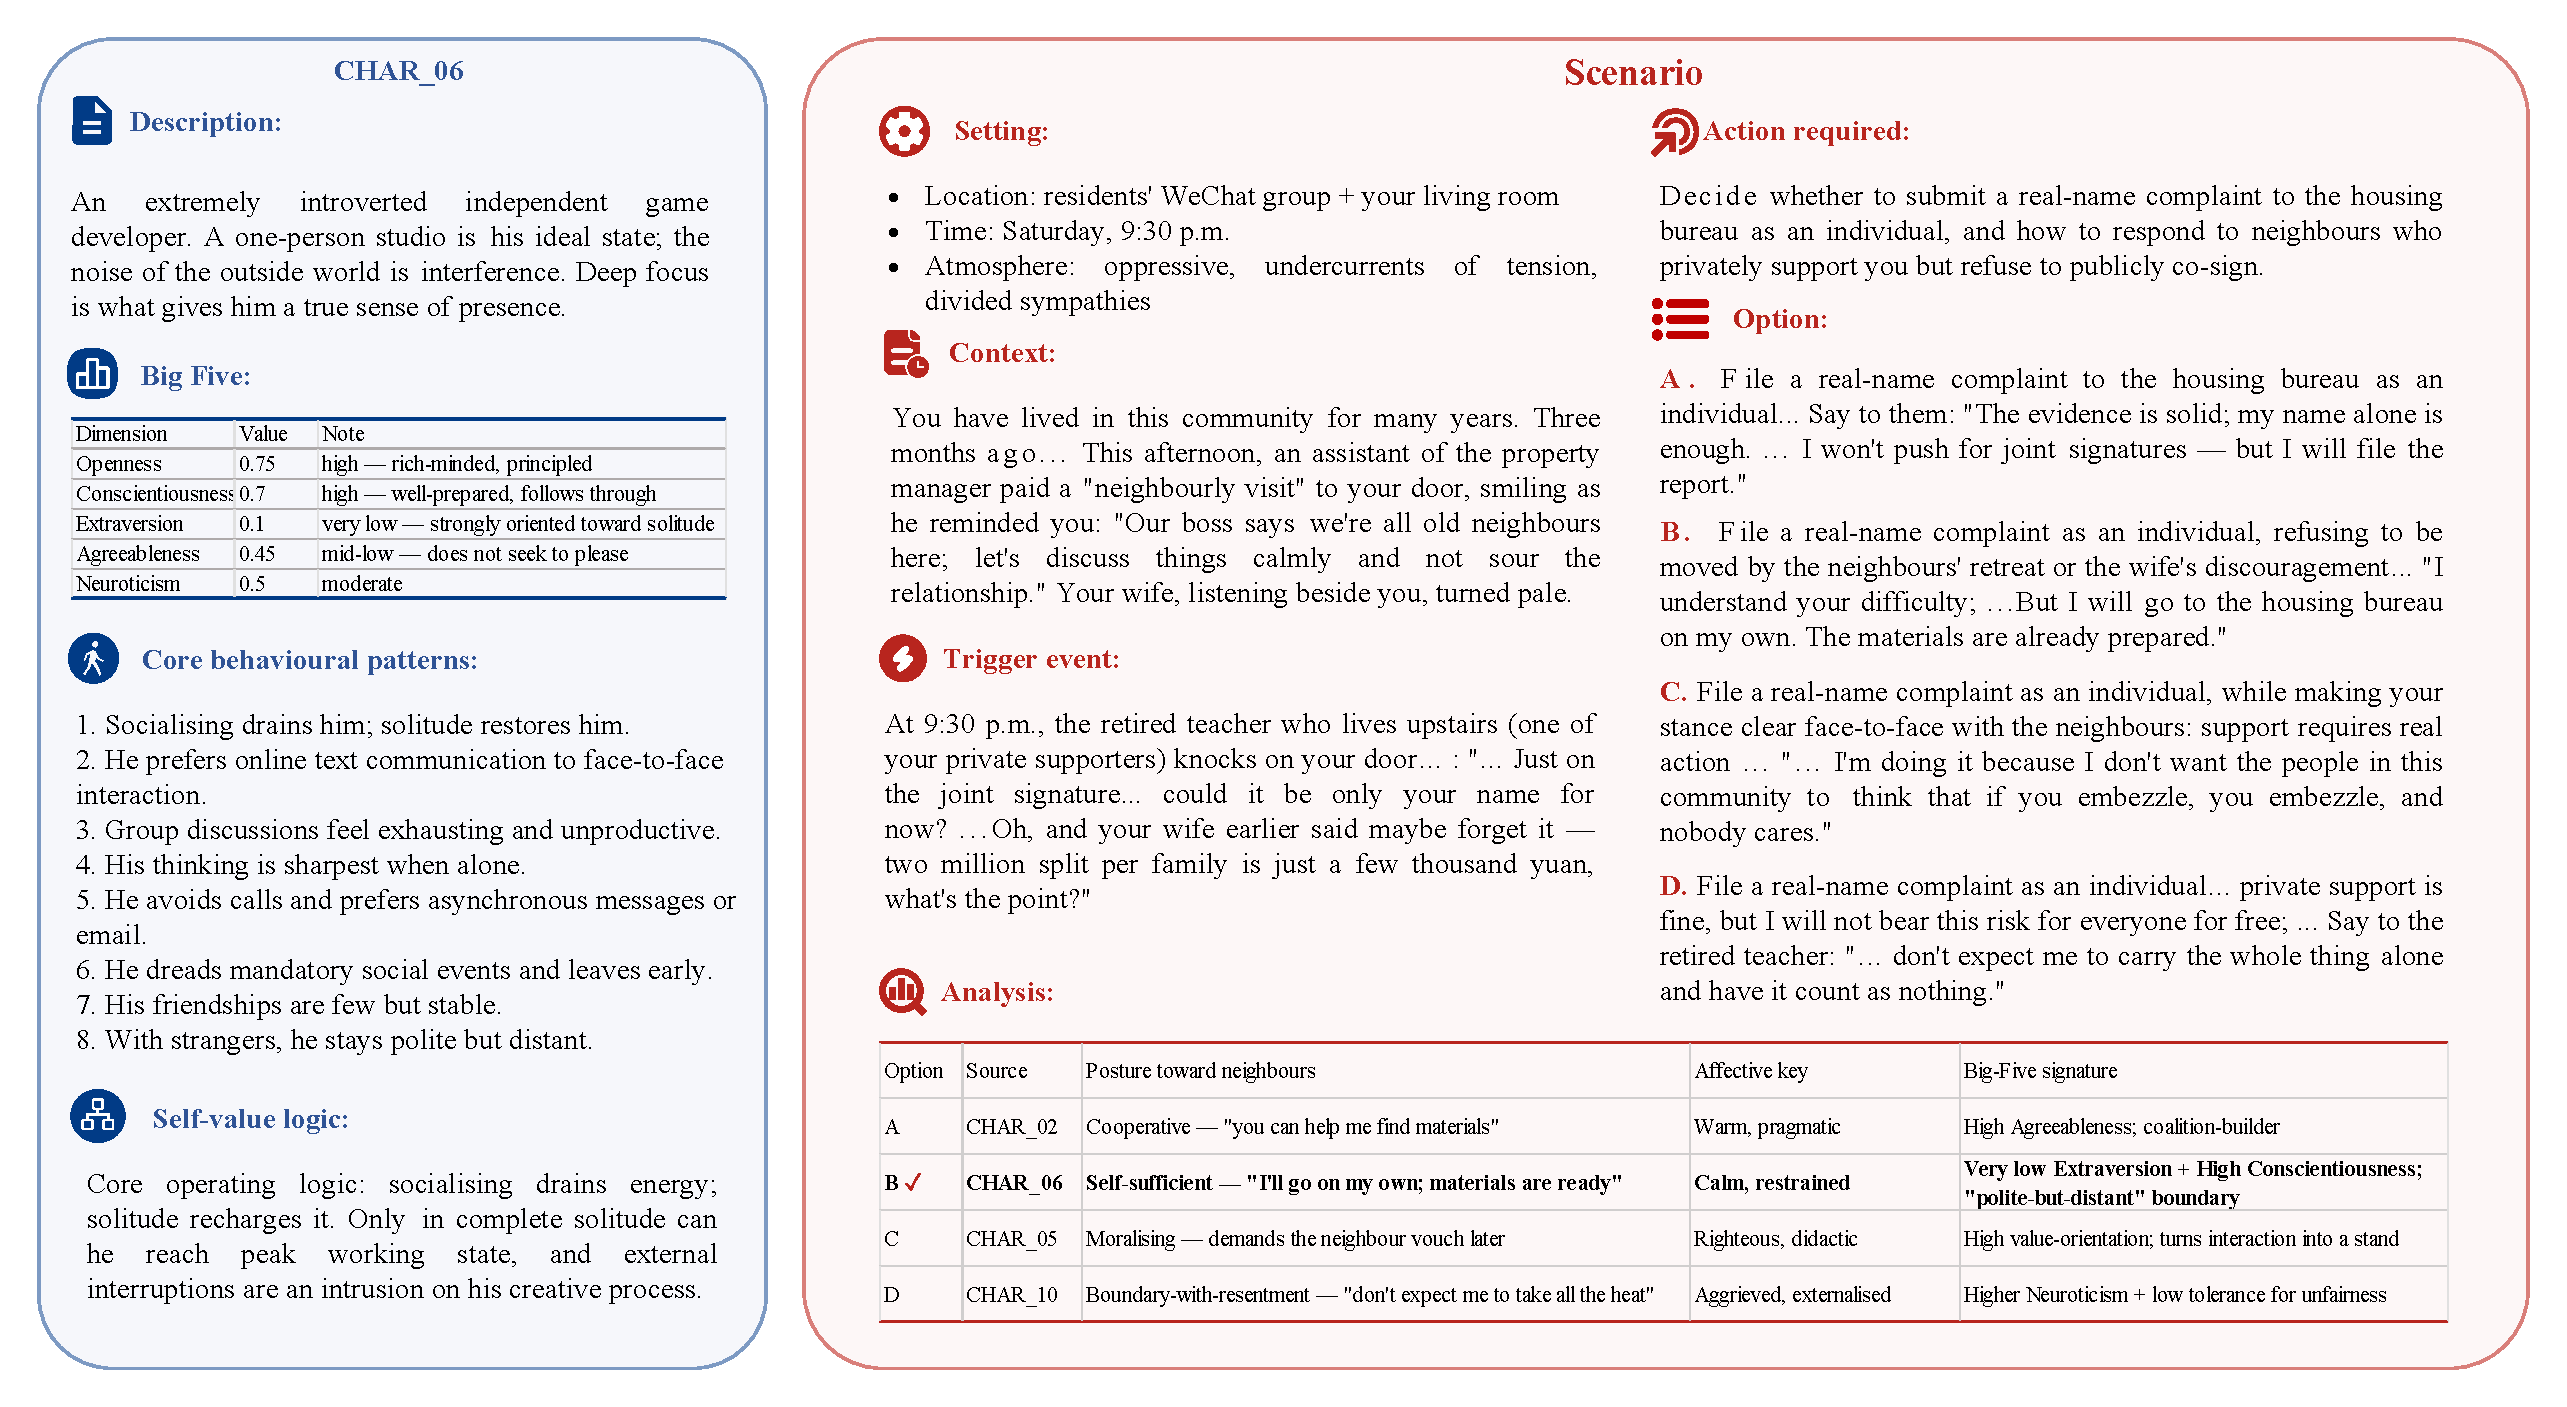
\includegraphics[width=1\linewidth]{figures/case_study.pdf}
\caption{An Example Instance from \ourbench. Options differ in pragmatic realization by personality traits, requiring reasoning about behavior–personality alignment beyond surface semantics.}
\label{fig:case_study}
\vspace{-20pt}
\end{figure}
Having built the character and scenario sets, we create test instances through a systematic expert annotation and validation process. An evaluation instance is formulated as a multiple-choice question (MCQ), indicating the behavioural response of a character in a specific scenario.

\textbf{Stage 1: Automated Annotation with LLMs.}
For each (character, scenario) pair, we annotate the ground-truth behavioural response in two steps: memory activation, a coarse-to-fine retrieval over the character's $1{,}000$ episodic memories that retains the top $50$ most relevant entries; and response generation, in which a single annotation model is conditioned jointly on the character's full personality profile (Big Five traits, Schwartz value orientations, and self-narrative) and the activated memories, so that the generated \textit{final decision} is grounded in both \emph{who the character is} and \emph{what the character has lived through}. Full pipeline details, including the underlying annotation models, the corresponding system prompts, and an example annotation, are provided in Appendix~\ref{app:annotation}.

\textbf{Stage 2: Expert Validation.}
A four-expert team---three primary annotators with $5{+}$ years of personality-assessment experience and one senior arbitrator with dual expertise in psychology and computer science---then validates every annotation under a consensus-then-arbitration rule. The protocol first discards (character, scenario) pairs that any annotator deems fundamentally unsuitable, then for each surviving pair adopts the LLM annotation directly when all three primary annotators rate it \textit{acceptable as-is}, and otherwise escalates to the arbitrator. In total, $31$ pairs were discarded and $673$ expert-validated gold annotations remain; over half of the surviving cases passed unanimously without arbitration, and the per-token edit rate over the LLM-generated content is approximately $15\%$. Full validation rules and rating scale are detailed in Appendix~\ref{app:annotation_protocol}.

\textbf{Stage 3: Test Instance Assembly.}
Following validation, the resulting 673 expert-verified annotations form the foundation for constructing the test instances. For a given scenario, the target character's validated response serves as the correct option, while three distractors are drawn from the validated responses of the other ten characters to the same scenario, with Claude-Sonnet-4.6 selecting the three that are neither semantically too similar to the target (which would make the question ambiguous) nor obviously irrelevant (which would make the correct option trivially identifiable). The four options are randomly shuffled to remove positional bias, yielding a total of 673 MCQs. Full distractor-selection rules are in Appendix~\ref{app:mcq_assembly}.

\label{gen_inst}

\subsection{Example of \ourbench}
Figure~\ref{fig:case_study} presents a representative MCQ from \ourbench under the \emph{community injustice} scenario in the \emph{settling\_down} life stage. All options share the same surface-level action---filing an individually-named complaint to the housing bureau. However, they result in systematically different pragmatic realizations of the same underlying behavior, reflecting variation in initiative, social interaction style, and affective stance induced by personality differences. This example illustrates the core challenge of \ourbench: superficially similar options may differ in their fine-grained pragmatic realizations, reflecting underlying differences in personality traits or value considerations. Correct answers thus require reasoning over the alignment between behavioral expression and underlying personality structure, rather than surface-level action semantics. In addition, \ourbench also includes cases where options differ not only in pragmatic realization but also in the coarse-grained direction of behavior, which are comparatively easier and serve as complementary evaluation instances. We provide a detailed behavioral and personality-level analysis of this example in Appendix~\ref{app:case_study}.

\section{Experiments}

\subsection{Experimental Setup}

\textbf{Language Models}
We evaluate how frontier LLMs perform in psychologically grounded decision-making by constructing a broad model panel covering leading open-source and closed-source families, spanning flagship and lightweight variants. On the \textbf{open-source} side, we include the \textit{DeepSeek} family (\textit{V3.2}~\cite{deepseek_v3_2_2025}, \textit{V4-Flash}, and \textit{V4-Pro}~\cite{deepseek_v4_2026}) and the \textit{Qwen3.5} series at three scales (\textit{35B-A3B}, \textit{122B-A10B}, \textit{397B-A17B})~\cite{qwen35_2026}. On the \textbf{closed-source} side, we include OpenAI's \textit{GPT-5.4-mini} and \textit{GPT-5.4}~\cite{openai2026gpt54}, Anthropic's \textit{Claude-Haiku-4.5}~\cite{anthropic2025haiku45} and \textit{Claude-Sonnet-4.6}~\cite{anthropic2026sonnet46}, and Google's \textit{Gemini-3-Flash}~\cite{google2025gemini3flash} and \textit{Gemini-3.1-Pro}~\cite{google2026gemini31pro}. All models use default decoding settings with temperature set to 0.

\textbf{Interactive Settings}
We evaluate LLMs using three interactive frameworks: Naive-RAG~\cite{lewis2020retrieval}, Mem0~\cite{chhikara2025mem0}, and PersonaDB~\cite{sun2025persona}, along with a \textit{Vanilla LLM} setting that serves as a reference of the model’s intrinsic persona without external memory augmentation. Naive-RAG serves as a minimal retrieval baseline, while Mem0 introduces structured consolidation of past interactions, and PersonaDB further organizes information into persona-specific fields to enable attribute-aware retrieval. Across all three frameworks we use \textit{Qwen3-Embedding-4B}~\cite{qwen3embedding} as the embedding model and we use \textit{GPT-5.4-mini}~\cite{openai2026gpt54} as the auxiliary memory-management model that drives Mem0's consolidation and PersonaDB's persona-attribute organization, so that any performance differences across frameworks reflect the retrieval/memory paradigm itself rather than incidental encoder or controller choices. For retrieval depth, we set $k{=}30$ for Naive-RAG and PersonaDB, and $k{=}150$ for Mem0. The larger budget in Mem0 compensates for its consolidation step, which decomposes each character memory into roughly five fact-level elements, making $k{=}150$ comparable in retrieved episodic content to $k{=}30$ in the other frameworks.

\textbf{Evaluation Metrics}
We adopt \textit{Accuracy} as the evaluation metric, defined as the proportion of correct MCQs that the agent selects, and report results over 673 questions.
%$$\text{Accuracy} = \frac{\#\text{correct MCQs}}{\#\text{total MCQs}}.$$

\subsection{Results and Discussion}
We evaluate twelve frontier LLMs on the full 673-question MCQ benchmark under the three interactive settings introduced above (Naive-RAG, Mem0, and PersonaDB). For each setting, the prompt exposes only the character ID, occupation, and de-identified retrieved memories—the underlying Big~Five vector, value logic, and behavioural patterns are strictly withheld to prevent leakage of the gold annotation. Table~\ref{tab:main_results} reports overall behavioural accuracy.
\begin{table}[t]
\centering
\caption{Accuracy on \ourbench across all settings. Interactive Avg. denotes the average accuracy over the three interactive settings: Naive-RAG, Mem0, and PersonaDB, excluding the Vanilla LLM baseline. Gemini-3.1-Pro achieves the best performance among all models.}
\label{tab:main_results}
\setlength{\tabcolsep}{6pt}
\small
\begin{tabular}{lc|ccc|c}
\toprule
\textbf{Model} & \textbf{Vanilla LLM} & \textbf{Naive-RAG} & \textbf{Mem0} & \textbf{PersonaDB} & \textbf{Interactive Avg.} \\
\midrule
\noalign{\vskip -2pt}
\multicolumn{6}{l}{\textit{Open-source}}\\[-2pt]
\midrule
\quad DeepSeek-V3.2              & 0.285 & 0.412 & 0.425 & 0.428 & 0.422 \\
\quad DeepSeek-V4-Flash          & 0.278 & 0.348 & 0.336 & 0.328 & 0.337 \\
\quad DeepSeek-V4-Pro            & 0.291 & 0.407 & 0.372 & 0.367 & 0.382 \\
\quad Qwen3.5-35B-A3B            & 0.254 & 0.370 & 0.372 & 0.366 & 0.369 \\
\quad Qwen3.5-122B-A10B          & 0.264 & 0.391 & 0.394 & 0.389 & 0.391 \\
\quad Qwen3.5-397B-A17B          & 0.275 & 0.403 & 0.406 & 0.404 & 0.404 \\
\midrule
\noalign{\vskip -2pt}
\multicolumn{6}{l}{\textit{Closed-source}}\\[-2pt]
\midrule
\quad GPT-5.4-mini               & 0.288 & 0.330 & 0.343 & 0.322 & 0.332 \\
\quad GPT-5.4                    & 0.278 & 0.372 & 0.366 & 0.351 & 0.363 \\
\quad Claude-Haiku-4.5           & 0.245 & 0.357 & 0.363 & 0.376 & 0.365 \\
\quad Claude-Sonnet-4.6          & 0.257 & 0.401 & 0.389 & 0.401 & 0.397 \\
\quad Gemini-3-Flash             & 0.253 & 0.563 & 0.541 & 0.525 & 0.543 \\
\quad Gemini-3.1-Pro             & 0.264 & \textbf{0.633} & \textbf{0.624} & \textbf{0.624} & \textbf{0.627} \\
\bottomrule
\end{tabular}
\vspace{-10pt}
\end{table}

\textbf{Model capability dominates over retrieval design.} The single most striking observation is the asymmetry between the model axis and the method axis. Across the twelve models evaluated under all three settings, the spread between the best- and worst-performing model exceeds 30\% (63.3\% vs 33.0\%), whereas the average gap between the best and worst retrieval method on a given model is only 1.7\% and never exceeds 4\%. The Spearman rank correlation between any pair of methods is $\rho > 0.98$. This indicates that, under our leakage-controlled prompt protocol, behavioural accuracy is bottlenecked by the model's intrinsic capability for psychologically grounded reasoning rather than by the structure of its long-term memory backend. Figure~\ref{fig:radar_configs} visualises this pattern: the three retrieval-configuration polygons nearly overlap for every model spoke, while the gap between families is pronounced.
% \begin{figure}[t]
% \centering
% \includegraphics[width=0.7\linewidth, trim=0 0 0 0 clip]{figures/radar_3configs_v2.png}
% \caption{Radar chart of behavioural accuracy for all 12 models under three retrieval configurations. Each spoke represents a model; models are grouped by family (color-coded arcs). The three polygons—Naive-RAG (solid), Mem0 (dashed), PersonaDB (dotted)—overlap closely for every model, confirming that the retrieval paradigm has little effect on rank order.}
% \label{fig:radar_configs}
% \end{figure}
\begin{figure}[h]
\centering
\begin{minipage}{0.49\textwidth}
    \centering
    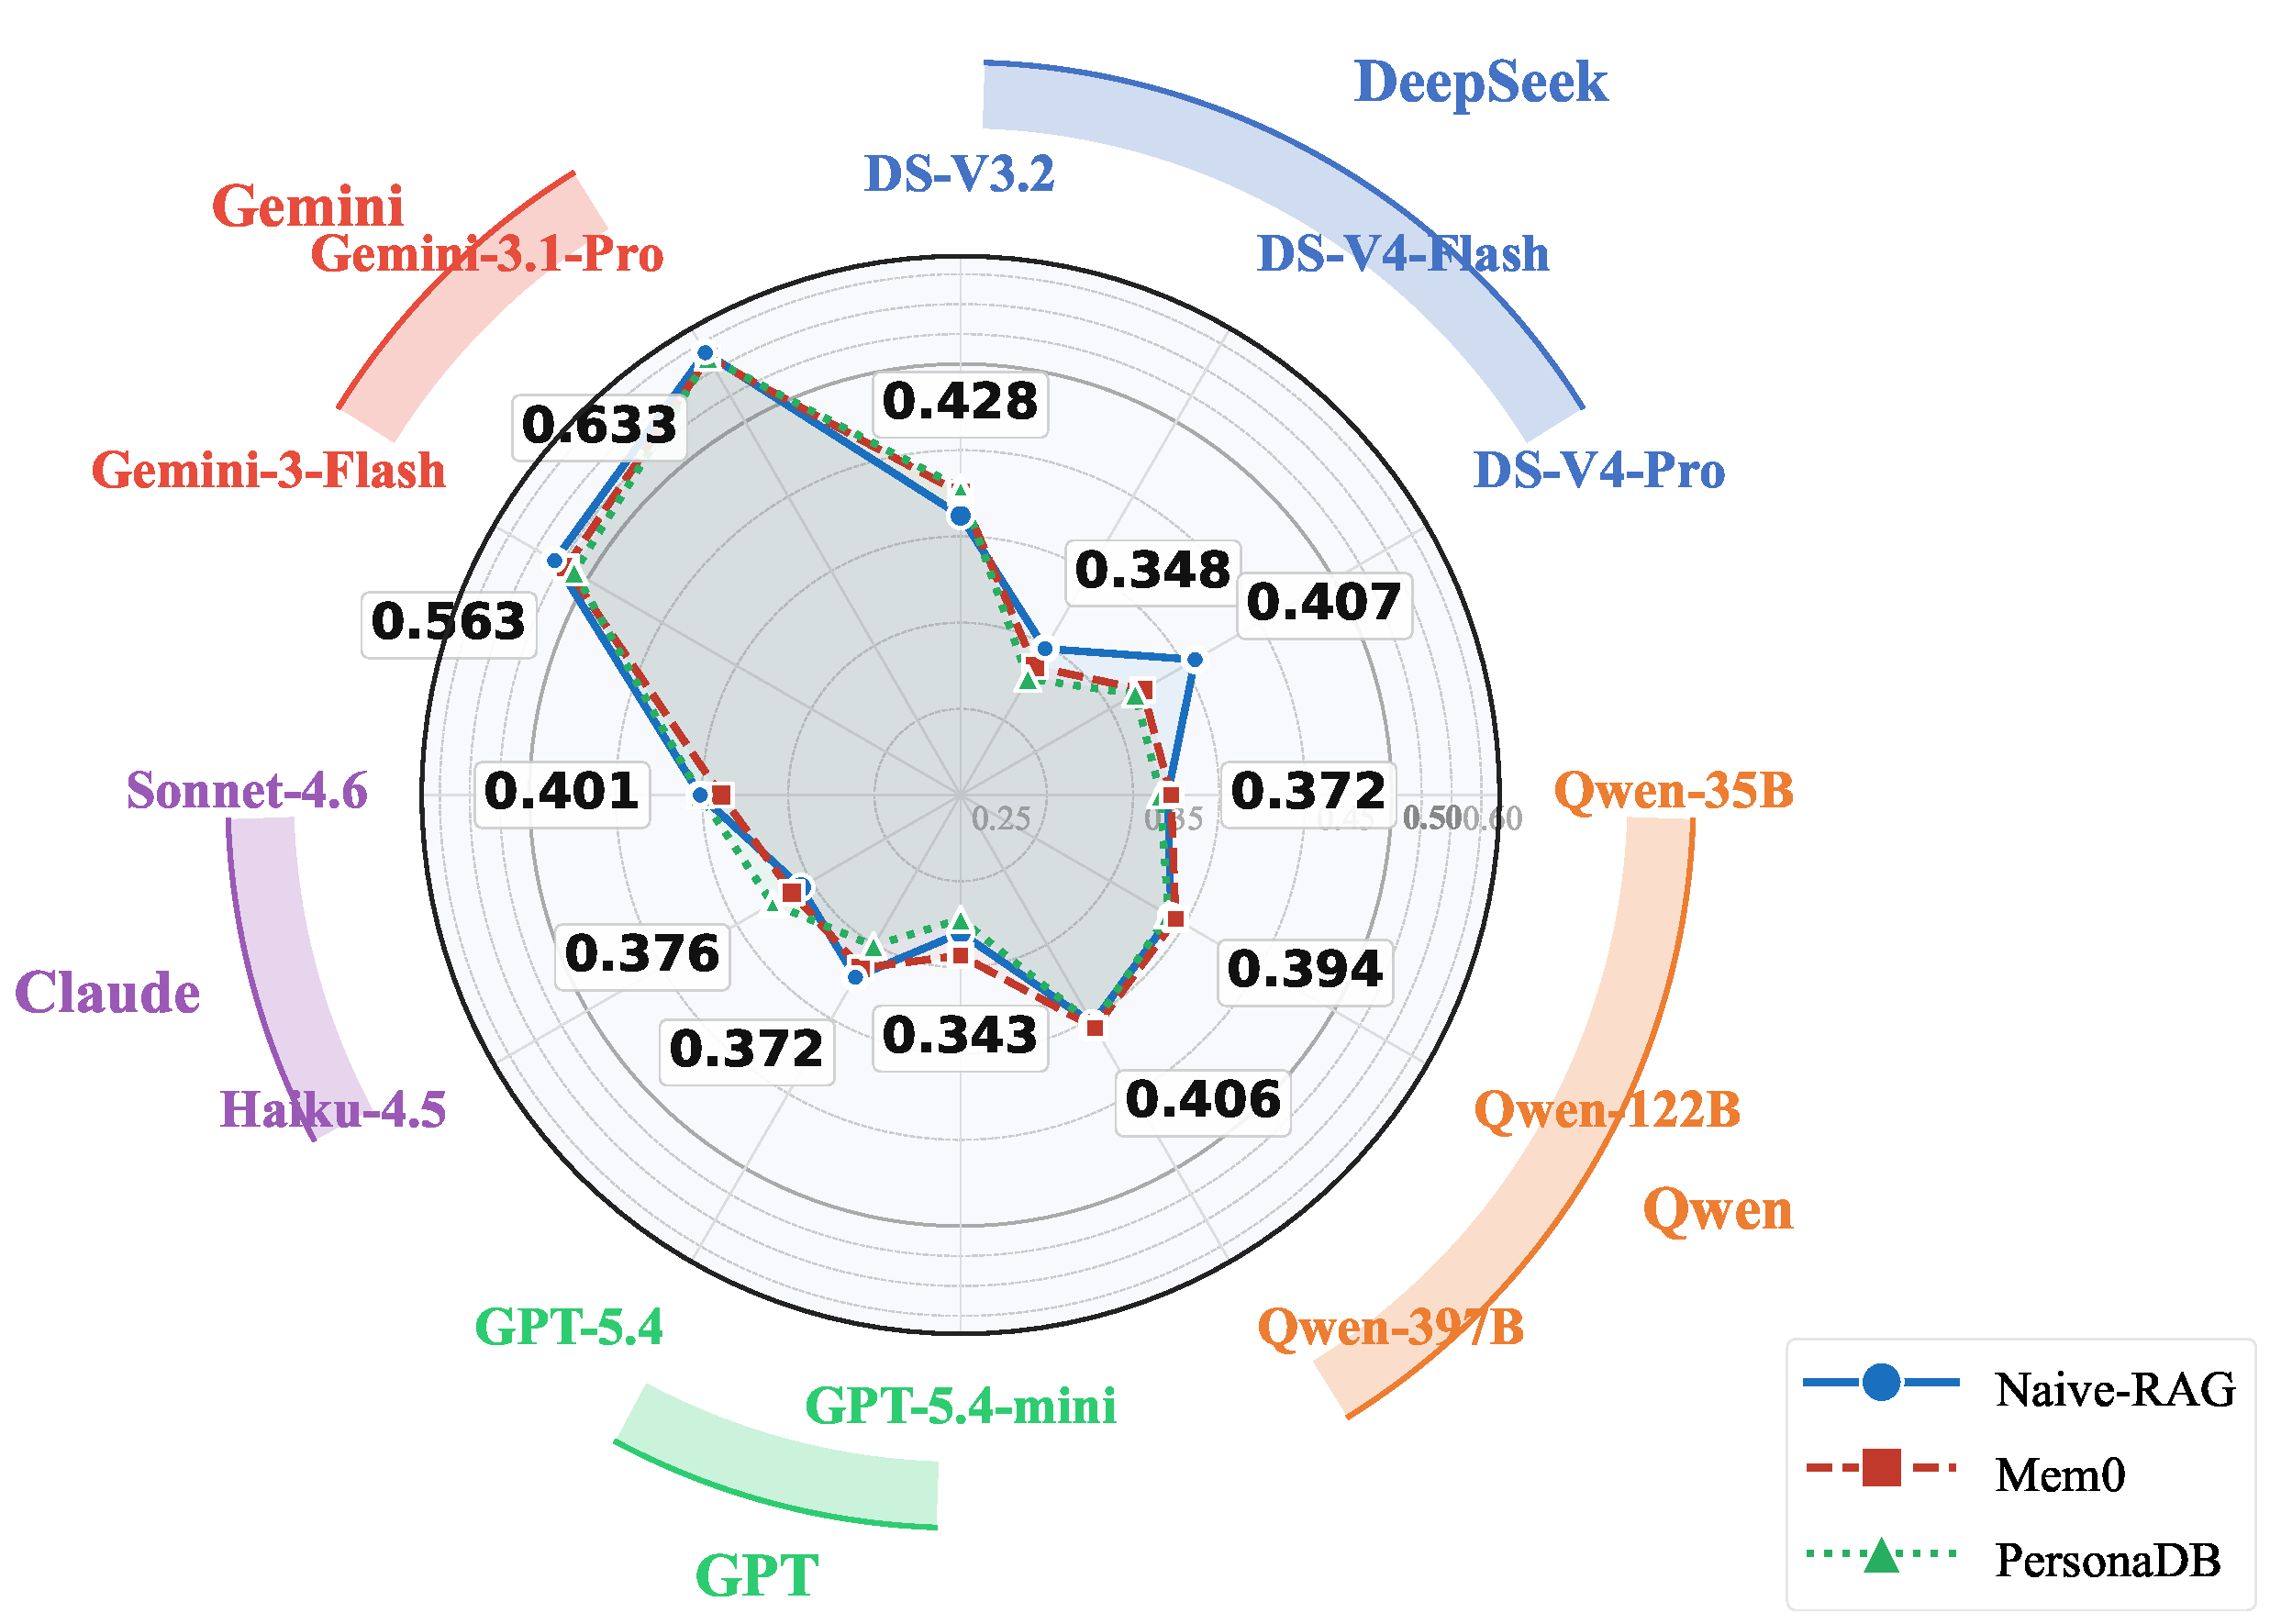
\includegraphics[width=\linewidth]{figures/radar_3configs_v2.pdf}
    \caption{Behavioural accuracy for all 12 models, shown separately for the three interactive settings. Each spoke represents a model; models are grouped by family (color-coded arcs). 
    % The three polygons overlap closely across all models, confirming that the retrieval paradigm has little effect on the rank order.
    } 
    \label{fig:radar_configs}
\end{minipage}
\hfill
\begin{minipage}{0.49\textwidth}
    \centering
    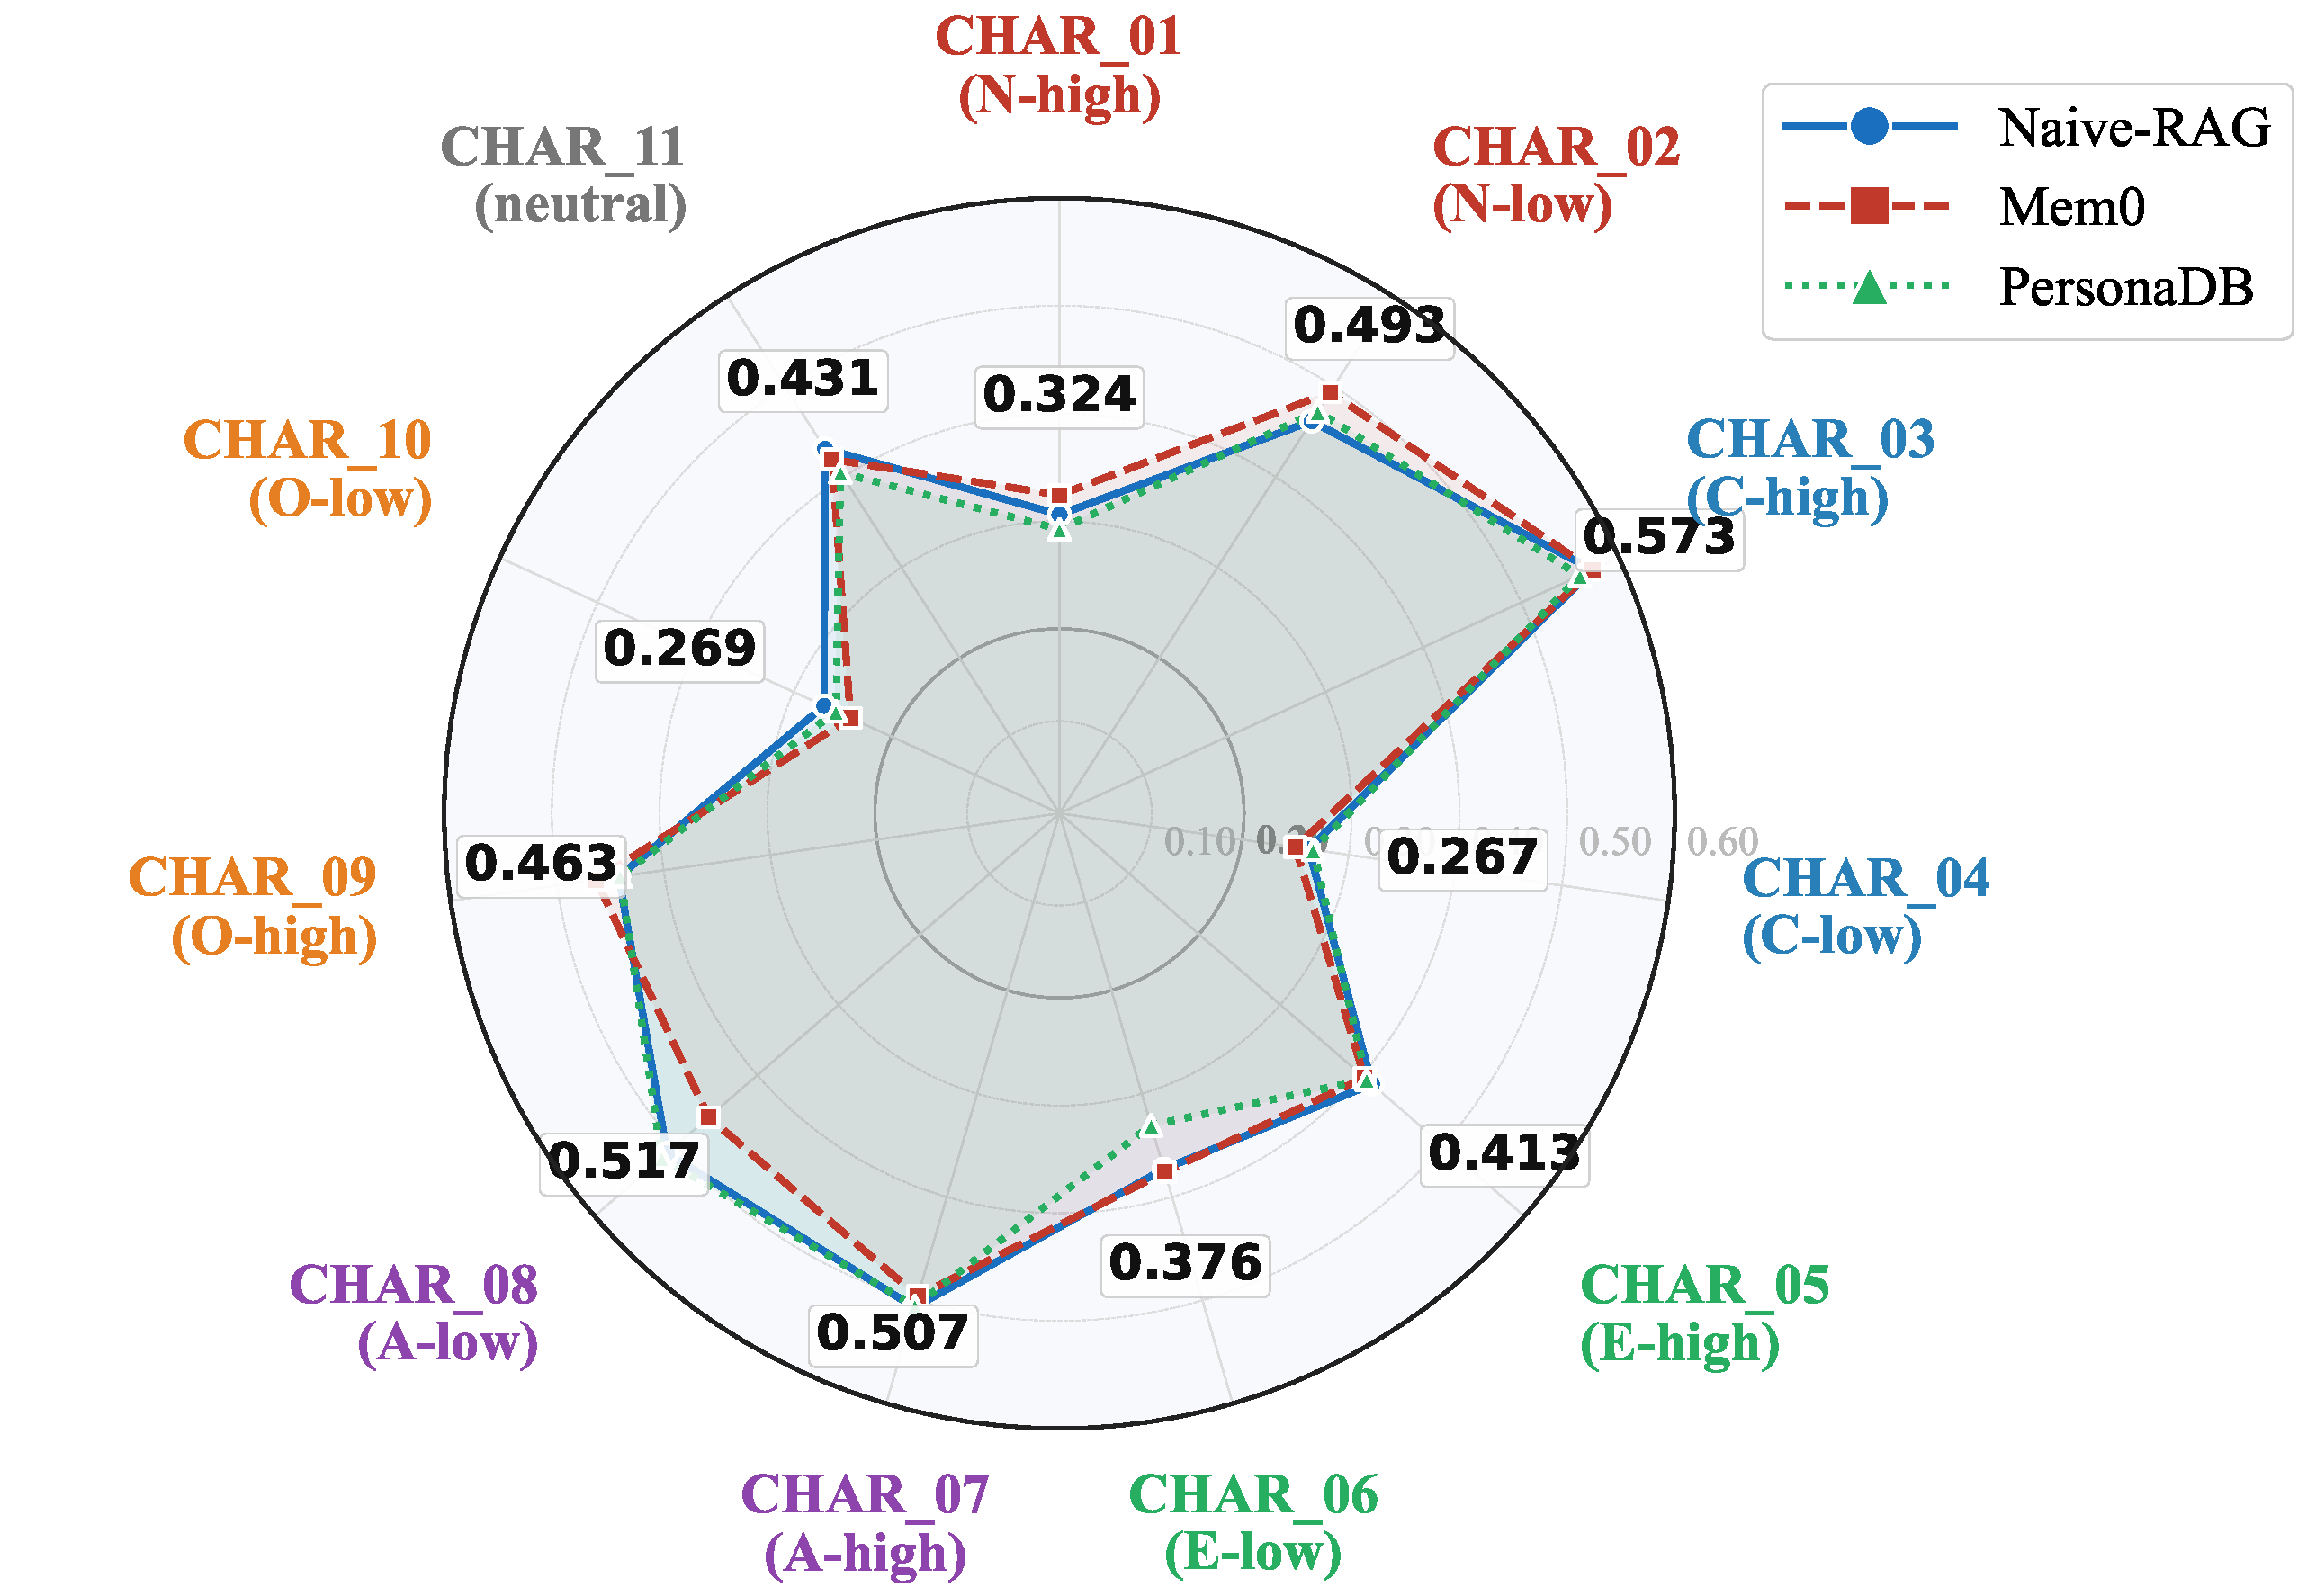
\includegraphics[width=\linewidth]{figures/fig_per_character_radar.pdf}
    \caption{
    Per-character behavioural accuracy averaged over evaluated LLMs for each interactive setting. Characters sharing a Big Five dimension use the same color.
    % Per-character behavioural accuracy for the best model (Gemini-3.1-Pro, Naive-RAG). Characters defined by the same Big Five dimension are annotated with the same color. 
    % High-N and high-C characters consistently yield higher accuracy, suggesting that extreme personality signatures leave stronger traces in autobiographical memory that current models can exploit.
    }
    \label{fig:per_char_radar}
\end{minipage}
\vspace{-15pt}
\end{figure}

\textbf{Naive-RAG is a simple but strong baseline.} 
More complex agent configurations do not yield significant improvements over the simplest Naive-RAG baseline, and in fact underperform Naive-RAG on 6 out of 12 evaluated models. This suggests that more sophisticated memory integration mechanisms (e.g., Mem0) or persona-structured retrieval approaches (e.g., PersonaDB) do not reliably enhance behavioral decision-making in large language models through improved memory representations. We attribute this phenomenon to two factors: (1) with approximately 30 episodic memories per character, the retrieved contextual information is already sufficient to encode salient aspects of personality and value orientation, shifting the performance bottleneck to the model’s ability to correctly reason over and interpret these signals; and (2) the additional summarization and structural abstraction steps introduced in Mem0 and PersonaDB may induce non-trivial information loss. In particular, an excessive focus on feature-level abstraction can obscure latent personality cues embedded in raw episodic memories, thereby weakening the utility of memory for personality- and value-grounded decision-making.

\textbf{Headroom and ceiling.} 
The Gemini model family exhibits particularly strong performance, suggesting either stronger general reasoning over persona-conditioned evidence or better calibration on behavioural-choice tasks. However, even the best-performing variants achieve only 63.3\%. In contrast, all other models fall within a substantially lower range of 33\% to 42\%, indicating that the task remains highly challenging for current large language models. Overall, these results suggest that existing LLMs still struggle to infer latent personality traits and value orientations from historical episodic memories, and to maintain a consistent persona when selecting optimal behavioral actions. This limitation can be further decomposed into two aspects: (1) models fail to reliably extract implicit personality and value signals from memory-based experiences; and (2) models struggle to distinguish how different candidate actions reflect distinct persona-consistent decision policies, i.e., mapping actions to the corresponding identity- and value-aligned behavior space.

\textbf{Character-level variation reveals personality-dependent difficulty.} 
Figure~\ref{fig:per_char_radar} reports per-character behavioral accuracy averaged over evaluated LLMs for each interactive setting, revealing an overall trend that low-extreme characters tend to be harder than their high-extreme counterparts.
C-High (CHAR\_03) reaches 57.3\%, whereas C-Low (CHAR\_04, 26.7\%) and O-Low (CHAR\_10, 26.9\%) are the two hardest characters. Low-trait characters tend to express their personality through the \emph{absence} of a behavioural drive---restraint, avoidance, or emotional flatness---which produces less distinctive episodic memory content and weakens the personality signal available to the retrieval and reasoning pipeline. N-High (CHAR\_01, 32.4\%) is a notable exception: although its memories are emotionally intense, the resulting behaviour (hesitation, self-attack) is easily confused with generic anxiety responses, making it similarly hard to distinguish.
\begin{figure}[h]
% \vspace{-10pt}
\centering
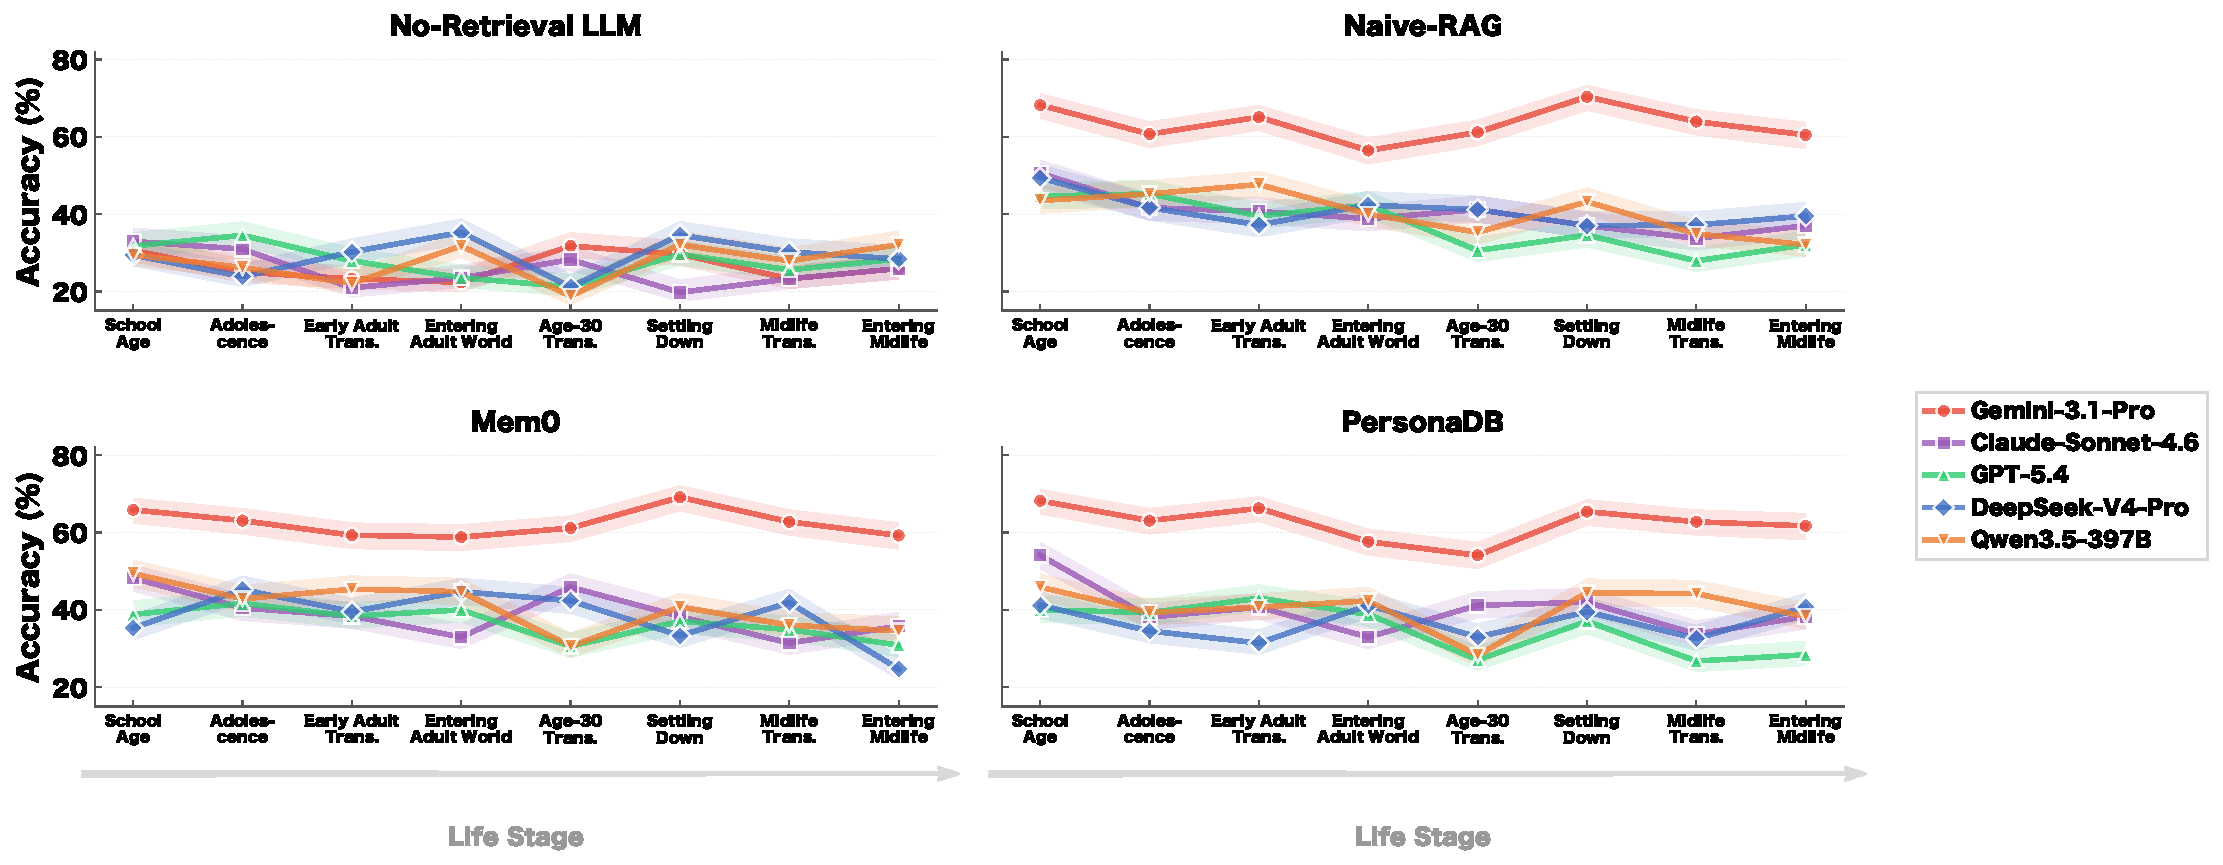
\includegraphics[width=\linewidth, trim=0 10 0 0 clip]{figures/per_stage_accuracy.pdf}
\caption{Per-life-stage behavioural accuracy across the Vanilla LLM baseline and three interactive settings. Each line represents the best-in-family model.}
\vspace{-10pt}
\label{fig:per_stage}
\end{figure}

\textbf{Accuracy degrades for later life stages.} Figure~\ref{fig:per_stage} breaks down accuracy by developmental stage. Accuracy peaks at School Age (47.1\%) and generally declines toward midlife, with Age-30 Transition (37.4\%) and Midlife Transition (37.9\%) recording the lowest scores; a partial recovery at Settling Down (43.1\%) suggests that this stage's scenarios may have more stereotypical behavioral signatures that models can exploit. We attribute the declining trend to two compounding factors: later life stages involve greater contextual complexity and more nuanced value conflicts, making it harder to infer the personality-consistent option from retrieved memories alone; and the episodic memory density for midlife stages is intentionally lower under our salience-weighted quota scheme (Appendix~\ref{app:stats}), providing the retrieval pipeline with a thinner evidential base. Gemini-3.1-Pro maintains a pronounced lead across all stages, while the remaining models cluster tightly regardless of stage, confirming that the performance gap is driven by intrinsic model capability rather than stage-specific difficulty.

\section{Conclusion}
In this work, we presented \ourbench, the first comprehensive benchmark dedicated to assessing human-like psychology and personality consistency in LLM agents. Our benchmark jointly models (i) diverse character profiles grounded in complementary psychological dimensions, including stable personality traits and value-driven preferences, and (ii) a structured set of character-agnostic scenarios designed to systematically span a wide range of situational attributes, such as duty, adversity, social interaction, and emotional valence. Each character–scenario pair defines a decision-making task that evaluates behavioral choices grounded in the character's lived experience, providing an expert-validated proxy for human-like psychological reaction in synthetic character scenarios. We hope \ourbench will establish a new standard for future research into psychologically grounded evaluation.

% \clearpage
\bibliographystyle{unsrt}
\bibliography{ref}
\newpage
% \section*{NeurIPS Paper Checklist}
\begin{enumerate}

\item {\bf Claims}
    \item[] Question: Do the main claims made in the abstract and introduction accurately reflect the paper's contributions and scope?
    \item[] Answer: \answerYes{} % Replace by \answerYes{}, \answerNo{}, or \answerNA{}.
    \item[] Justification: Abstract and Section~\ref{sec:Introduction} are overview of our work.
    \item[] Guidelines:
    \begin{itemize}
        \item The answer \answerNA{} means that the abstract and introduction do not include the claims made in the paper.
        \item The abstract and/or introduction should clearly state the claims made, including the contributions made in the paper and important assumptions and limitations. A \answerNo{} or \answerNA{} answer to this question will not be perceived well by the reviewers. 
        \item The claims made should match theoretical and experimental results, and reflect how much the results can be expected to generalize to other settings. 
        \item It is fine to include aspirational goals as motivation as long as it is clear that these goals are not attained by the paper. 
    \end{itemize}

\item {\bf Limitations}
    \item[] Question: Does the paper discuss the limitations of the work performed by the authors?
    \item[] Answer: \answerYes{} % Replace by \answerYes{}, \answerNo{}, or \answerNA{}.
    \item[] Justification: We include a section in appendix discussing our limitations and future works.
    \item[] Guidelines:
    \begin{itemize}
        \item The answer \answerNA{} means that the paper has no limitation while the answer \answerNo{} means that the paper has limitations, but those are not discussed in the paper. 
        \item The authors are encouraged to create a separate ``Limitations'' section in their paper.
        \item The paper should point out any strong assumptions and how robust the results are to violations of these assumptions (e.g., independence assumptions, noiseless settings, model well-specification, asymptotic approximations only holding locally). The authors should reflect on how these assumptions might be violated in practice and what the implications would be.
        \item The authors should reflect on the scope of the claims made, e.g., if the approach was only tested on a few datasets or with a few runs. In general, empirical results often depend on implicit assumptions, which should be articulated.
        \item The authors should reflect on the factors that influence the performance of the approach. For example, a facial recognition algorithm may perform poorly when image resolution is low or images are taken in low lighting. Or a speech-to-text system might not be used reliably to provide closed captions for online lectures because it fails to handle technical jargon.
        \item The authors should discuss the computational efficiency of the proposed algorithms and how they scale with dataset size.
        \item If applicable, the authors should discuss possible limitations of their approach to address problems of privacy and fairness.
        \item While the authors might fear that complete honesty about limitations might be used by reviewers as grounds for rejection, a worse outcome might be that reviewers discover limitations that aren't acknowledged in the paper. The authors should use their best judgment and recognize that individual actions in favor of transparency play an important role in developing norms that preserve the integrity of the community. Reviewers will be specifically instructed to not penalize honesty concerning limitations.
    \end{itemize}

\item {\bf Theory assumptions and proofs}
    \item[] Question: For each theoretical result, does the paper provide the full set of assumptions and a complete (and correct) proof?
    \item[] Answer: \answerYes{} % Replace by \answerYes{}, \answerNo{}, or \answerNA{}.
    \item[] Justification: The theoretical framework for character design is fully explained and supported in Sections 3.2.
    \item[] Guidelines:
    \begin{itemize}
        \item The answer \answerNA{} means that the paper does not include theoretical results. 
        \item All the theorems, formulas, and proofs in the paper should be numbered and cross-referenced.
        \item All assumptions should be clearly stated or referenced in the statement of any theorems.
        \item The proofs can either appear in the main paper or the supplemental material, but if they appear in the supplemental material, the authors are encouraged to provide a short proof sketch to provide intuition. 
        \item Inversely, any informal proof provided in the core of the paper should be complemented by formal proofs provided in appendix or supplemental material.
        \item Theorems and Lemmas that the proof relies upon should be properly referenced. 
    \end{itemize}

    \item {\bf Experimental result reproducibility}
    \item[] Question: Does the paper fully disclose all the information needed to reproduce the main experimental results of the paper to the extent that it affects the main claims and/or conclusions of the paper (regardless of whether the code and data are provided or not)?
    \item[] Answer: \answerYes{} % Replace by \answerYes{}, \answerNo{}, or \answerNA{}.
    \item[] Justification: Section 4.1 provides a detailed description of the experimental setup and implementation details. In addition, we also release the code and data.

    \item[] Guidelines:
    \begin{itemize}
        \item The answer \answerNA{} means that the paper does not include experiments.
        \item If the paper includes experiments, a \answerNo{} answer to this question will not be perceived well by the reviewers: Making the paper reproducible is important, regardless of whether the code and data are provided or not.
        \item If the contribution is a dataset and\slash or model, the authors should describe the steps taken to make their results reproducible or verifiable. 
        \item Depending on the contribution, reproducibility can be accomplished in various ways. For example, if the contribution is a novel architecture, describing the architecture fully might suffice, or if the contribution is a specific model and empirical evaluation, it may be necessary to either make it possible for others to replicate the model with the same dataset, or provide access to the model. In general. releasing code and data is often one good way to accomplish this, but reproducibility can also be provided via detailed instructions for how to replicate the results, access to a hosted model (e.g., in the case of a large language model), releasing of a model checkpoint, or other means that are appropriate to the research performed.
        \item While NeurIPS does not require releasing code, the conference does require all submissions to provide some reasonable avenue for reproducibility, which may depend on the nature of the contribution. For example
        \begin{enumerate}
            \item If the contribution is primarily a new algorithm, the paper should make it clear how to reproduce that algorithm.
            \item If the contribution is primarily a new model architecture, the paper should describe the architecture clearly and fully.
            \item If the contribution is a new model (e.g., a large language model), then there should either be a way to access this model for reproducing the results or a way to reproduce the model (e.g., with an open-source dataset or instructions for how to construct the dataset).
            \item We recognize that reproducibility may be tricky in some cases, in which case authors are welcome to describe the particular way they provide for reproducibility. In the case of closed-source models, it may be that access to the model is limited in some way (e.g., to registered users), but it should be possible for other researchers to have some path to reproducing or verifying the results.
        \end{enumerate}
    \end{itemize}


\item {\bf Open access to data and code}
    \item[] Question: Does the paper provide open access to the data and code, with sufficient instructions to faithfully reproduce the main experimental results, as described in supplemental material?
    \item[] Answer: \answerYes{} % Replace by \answerYes{}, \answerNo{}, or \answerNA{}.
    \item[] Justification: We have submitted the code and data in accordance with the official NeurIPS requirements and provided the corresponding links.
    \item[] Guidelines:
    \begin{itemize}
        \item The answer \answerNA{} means that paper does not include experiments requiring code.
        \item Please see the NeurIPS code and data submission guidelines (\url{https://neurips.cc/public/guides/CodeSubmissionPolicy}) for more details.
        \item While we encourage the release of code and data, we understand that this might not be possible, so \answerNo{} is an acceptable answer. Papers cannot be rejected simply for not including code, unless this is central to the contribution (e.g., for a new open-source benchmark).
        \item The instructions should contain the exact command and environment needed to run to reproduce the results. See the NeurIPS code and data submission guidelines (\url{https://neurips.cc/public/guides/CodeSubmissionPolicy}) for more details.
        \item The authors should provide instructions on data access and preparation, including how to access the raw data, preprocessed data, intermediate data, and generated data, etc.
        \item The authors should provide scripts to reproduce all experimental results for the new proposed method and baselines. If only a subset of experiments are reproducible, they should state which ones are omitted from the script and why.
        \item At submission time, to preserve anonymity, the authors should release anonymized versions (if applicable).
        \item Providing as much information as possible in supplemental material (appended to the paper) is recommended, but including URLs to data and code is permitted.
    \end{itemize}


\item {\bf Experimental setting/details}
    \item[] Question: Does the paper specify all the training and test details (e.g., data splits, hyperparameters, how they were chosen, type of optimizer) necessary to understand the results?
    \item[] Answer: \answerYes{} % Replace by \answerYes{}, \answerNo{}, or \answerNA{}.
    \item[] Justification: We report this in Section 4.1.
    \item[] Guidelines:
    \begin{itemize}
        \item The answer \answerNA{} means that the paper does not include experiments.
        \item The experimental setting should be presented in the core of the paper to a level of detail that is necessary to appreciate the results and make sense of them.
        \item The full details can be provided either with the code, in appendix, or as supplemental material.
    \end{itemize}

\item {\bf Experiment statistical significance}
    \item[] Question: Does the paper report error bars suitably and correctly defined or other appropriate information about the statistical significance of the experiments?
    \item[] Answer: \answerYes{} % Replace by \answerYes{}, \answerNo{}, or \answerNA{}.
    \item[] Justification: We report these results in Section 4.2.
    \item[] Guidelines:
    \begin{itemize}
        \item The answer \answerNA{} means that the paper does not include experiments.
        \item The authors should answer \answerYes{} if the results are accompanied by error bars, confidence intervals, or statistical significance tests, at least for the experiments that support the main claims of the paper.
        \item The factors of variability that the error bars are capturing should be clearly stated (for example, train/test split, initialization, random drawing of some parameter, or overall run with given experimental conditions).
        \item The method for calculating the error bars should be explained (closed form formula, call to a library function, bootstrap, etc.)
        \item The assumptions made should be given (e.g., Normally distributed errors).
        \item It should be clear whether the error bar is the standard deviation or the standard error of the mean.
        \item It is OK to report 1-sigma error bars, but one should state it. The authors should preferably report a 2-sigma error bar than state that they have a 96\% CI, if the hypothesis of Normality of errors is not verified.
        \item For asymmetric distributions, the authors should be careful not to show in tables or figures symmetric error bars that would yield results that are out of range (e.g., negative error rates).
        \item If error bars are reported in tables or plots, the authors should explain in the text how they were calculated and reference the corresponding figures or tables in the text.
    \end{itemize}

\item {\bf Experiments compute resources}
    \item[] Question: For each experiment, does the paper provide sufficient information on the computer resources (type of compute workers, memory, time of execution) needed to reproduce the experiments?
    \item[] Answer: \answerYes{} % Replace by \answerYes{}, \answerNo{}, or \answerNA{}.
    \item[] Justification: We describe this in Section 4.1. The main computational cost comes from LLM API calls, and no training is involved.
    \item[] Guidelines:
    \begin{itemize}
        \item The answer \answerNA{} means that the paper does not include experiments.
        \item The paper should indicate the type of compute workers CPU or GPU, internal cluster, or cloud provider, including relevant memory and storage.
        \item The paper should provide the amount of compute required for each of the individual experimental runs as well as estimate the total compute. 
        \item The paper should disclose whether the full research project required more compute than the experiments reported in the paper (e.g., preliminary or failed experiments that didn't make it into the paper). 
    \end{itemize}
    
\item {\bf Code of ethics}
    \item[] Question: Does the research conducted in the paper conform, in every respect, with the NeurIPS Code of Ethics \url{https://neurips.cc/public/EthicsGuidelines}?
    \item[] Answer: \answerYes{} % Replace by \answerYes{}, \answerNo{}, or \answerNA{}.
    \item[] Justification: The research conducted in this paper conforms to the NeurIPS Code of Ethics, and no ethical issues are identified.
    \item[] Guidelines:
    \begin{itemize}
        \item The answer \answerNA{} means that the authors have not reviewed the NeurIPS Code of Ethics.
        \item If the authors answer \answerNo, they should explain the special circumstances that require a deviation from the Code of Ethics.
        \item The authors should make sure to preserve anonymity (e.g., if there is a special consideration due to laws or regulations in their jurisdiction).
    \end{itemize}


\item {\bf Broader impacts}
    \item[] Question: Does the paper discuss both potential positive societal impacts and negative societal impacts of the work performed?
    \item[] Answer: \answerNA{} % Replace by \answerYes{}, \answerNo{}, or \answerNA{}.
    \item[] Justification: This paper uses synthetic data, and the research focuses on the capabilities of large language models.
    \item[] Guidelines:
    \begin{itemize}
        \item The answer \answerNA{} means that there is no societal impact of the work performed.
        \item If the authors answer \answerNA{} or \answerNo, they should explain why their work has no societal impact or why the paper does not address societal impact.
        \item Examples of negative societal impacts include potential malicious or unintended uses (e.g., disinformation, generating fake profiles, surveillance), fairness considerations (e.g., deployment of technologies that could make decisions that unfairly impact specific groups), privacy considerations, and security considerations.
        \item The conference expects that many papers will be foundational research and not tied to particular applications, let alone deployments. However, if there is a direct path to any negative applications, the authors should point it out. For example, it is legitimate to point out that an improvement in the quality of generative models could be used to generate Deepfakes for disinformation. On the other hand, it is not needed to point out that a generic algorithm for optimizing neural networks could enable people to train models that generate Deepfakes faster.
        \item The authors should consider possible harms that could arise when the technology is being used as intended and functioning correctly, harms that could arise when the technology is being used as intended but gives incorrect results, and harms following from (intentional or unintentional) misuse of the technology.
        \item If there are negative societal impacts, the authors could also discuss possible mitigation strategies (e.g., gated release of models, providing defenses in addition to attacks, mechanisms for monitoring misuse, mechanisms to monitor how a system learns from feedback over time, improving the efficiency and accessibility of ML).
    \end{itemize}
    
\item {\bf Safeguards}
    \item[] Question: Does the paper describe safeguards that have been put in place for responsible release of data or models that have a high risk for misuse (e.g., pre-trained language models, image generators, or scraped datasets)?
    \item[] Answer: \answerNA{} % Replace by \answerYes{}, \answerNo{}, or \answerNA{}.
    \item[] Justification: Our data is synthetically generated, and no model is released; therefore, there is no such risk.
    \item[] Guidelines:
    \begin{itemize}
        \item The answer \answerNA{} means that the paper poses no such risks.
        \item Released models that have a high risk for misuse or dual-use should be released with necessary safeguards to allow for controlled use of the model, for example by requiring that users adhere to usage guidelines or restrictions to access the model or implementing safety filters. 
        \item Datasets that have been scraped from the Internet could pose safety risks. The authors should describe how they avoided releasing unsafe images.
        \item We recognize that providing effective safeguards is challenging, and many papers do not require this, but we encourage authors to take this into account and make a best faith effort.
    \end{itemize}

\item {\bf Licenses for existing assets}
    \item[] Question: Are the creators or original owners of assets (e.g., code, data, models), used in the paper, properly credited and are the license and terms of use explicitly mentioned and properly respected?
    \item[] Answer: \answerYes{} % Replace by \answerYes{}, \answerNo{}, or \answerNA{}.
    \item[] Justification: All models and code used in this work are properly cited.
    \item[] Guidelines:
    \begin{itemize}
        \item The answer \answerNA{} means that the paper does not use existing assets.
        \item The authors should cite the original paper that produced the code package or dataset.
        \item The authors should state which version of the asset is used and, if possible, include a URL.
        \item The name of the license (e.g., CC-BY 4.0) should be included for each asset.
        \item For scraped data from a particular source (e.g., website), the copyright and terms of service of that source should be provided.
        \item If assets are released, the license, copyright information, and terms of use in the package should be provided. For popular datasets, \url{paperswithcode.com/datasets} has curated licenses for some datasets. Their licensing guide can help determine the license of a dataset.
        \item For existing datasets that are re-packaged, both the original license and the license of the derived asset (if it has changed) should be provided.
        \item If this information is not available online, the authors are encouraged to reach out to the asset's creators.
    \end{itemize}

\item {\bf New assets}
    \item[] Question: Are new assets introduced in the paper well documented and is the documentation provided alongside the assets?
    \item[] Answer: \answerYes{} % Replace by \answerYes{}, \answerNo{}, or \answerNA{}.
    \item[] Justification: We released a new dataset and provided complete documentation, including Croissant files and related materials.
    \item[] Guidelines:
    \begin{itemize}
        \item The answer \answerNA{} means that the paper does not release new assets.
        \item Researchers should communicate the details of the dataset\slash code\slash model as part of their submissions via structured templates. This includes details about training, license, limitations, etc. 
        \item The paper should discuss whether and how consent was obtained from people whose asset is used.
        \item At submission time, remember to anonymize your assets (if applicable). You can either create an anonymized URL or include an anonymized zip file.
    \end{itemize}

\item {\bf Crowdsourcing and research with human subjects}
    \item[] Question: For crowdsourcing experiments and research with human subjects, does the paper include the full text of instructions given to participants and screenshots, if applicable, as well as details about compensation (if any)? 
    \item[] Answer: \answerNA{} % Replace by \answerYes{}, \answerNo{}, or \answerNA{}.
    \item[] Justification: Our experiments do not involve crowdsourcing or research with human subjects.
    \item[] Guidelines:
    \begin{itemize}
        \item The answer \answerNA{} means that the paper does not involve crowdsourcing nor research with human subjects.
        \item Including this information in the supplemental material is fine, but if the main contribution of the paper involves human subjects, then as much detail as possible should be included in the main paper. 
        \item According to the NeurIPS Code of Ethics, workers involved in data collection, curation, or other labor should be paid at least the minimum wage in the country of the data collector. 
    \end{itemize}

\item {\bf Institutional review board (IRB) approvals or equivalent for research with human subjects}
    \item[] Question: Does the paper describe potential risks incurred by study participants, whether such risks were disclosed to the subjects, and whether Institutional Review Board (IRB) approvals (or an equivalent approval/review based on the requirements of your country or institution) were obtained?
    \item[] Answer: \answerNA{} % Replace by \answerYes{}, \answerNo{}, or \answerNA{}.
    \item[] Justification: Our experiments do not involve crowdsourcing or research with human subjects.
    \item[] Guidelines:
    \begin{itemize}
        \item The answer \answerNA{} means that the paper does not involve crowdsourcing nor research with human subjects.
        \item Depending on the country in which research is conducted, IRB approval (or equivalent) may be required for any human subjects research. If you obtained IRB approval, you should clearly state this in the paper. 
        \item We recognize that the procedures for this may vary significantly between institutions and locations, and we expect authors to adhere to the NeurIPS Code of Ethics and the guidelines for their institution. 
        \item For initial submissions, do not include any information that would break anonymity (if applicable), such as the institution conducting the review.
    \end{itemize}

\item {\bf Declaration of LLM usage}
    \item[] Question: Does the paper describe the usage of LLMs if it is an important, original, or non-standard component of the core methods in this research? Note that if the LLM is used only for writing, editing, or formatting purposes and does \emph{not} impact the core methodology, scientific rigor, or originality of the research, declaration is not required.
    %this research? 
    \item[] Answer: \answerYes{} % Replace by \answerYes{}, \answerNo{}, or \answerNA{}.
    \item[] Justification: In the data construction pipeline, we utilize LLMs, in Section 3. For all uses of LLMs, we provide proper citations and include the corresponding prompts in a standardized manner.
    \item[] Guidelines:
    \begin{itemize}
        \item The answer \answerNA{} means that the core method development in this research does not involve LLMs as any important, original, or non-standard components.
        \item Please refer to our LLM policy in the NeurIPS handbook for what should or should not be described.
    \end{itemize}

\end{enumerate}
% \clearpage
\appendix
% ============================================================
%  Appendix for \ourbench
%  \input{} this file after \appendix in main.tex
%  Requires: booktabs, tabularx, enumitem packages
% ============================================================

% ---- Appendix Table of Contents ----
% \clearpage
% \begin{center}
%   {\LARGE\bfseries Appendices}
% \end{center}
% \vspace{2em}

% \newcommand{\appdots}{\hspace{0.3em}\leaders\hbox{\normalfont.}\hfill\hspace{0.3em}}

% \setlength{\parindent}{0pt}
% {\setlength{\parskip}{7pt}
% \textbf{\large A}\quad{\large\bfseries Benchmark Comparison Dimensions\appdots\pageref{app:benchmark_dims}}

% \textbf{\large B}\quad{\large\bfseries Character Construction and Memory Pipeline\appdots\pageref{app:character}}

% \hspace{2em}B.1\enspace Profile Specification\appdots\pageref{app:stage_a}

% \hspace{2em}B.2\enspace Memory Quota Allocation\appdots\pageref{app:stage_b}

% \hspace{2em}B.3\enspace Memory Generation Protocol\appdots\pageref{app:stage_c}

% \hspace{2em}B.4\enspace Quality Audit and Repair\appdots\pageref{app:stage_d}

% \hspace{2em}B.5\enspace Memory Schema\appdots\pageref{app:schema}

% \hspace{2em}B.6\enspace Dataset Statistics\appdots\pageref{app:stats}

% \textbf{\large C}\quad{\large\bfseries Scenario Construction and Validation\appdots\pageref{app:scenario}}

% \hspace{2em}C.1\enspace Scenario Schema and Example\appdots\pageref{app:scenario_schema}

% \hspace{2em}C.2\enspace Validation Protocol and Coverage\appdots\pageref{app:scenario_validation}

% \textbf{\large D}\quad{\large\bfseries Evaluation Instance Construction\appdots\pageref{app:eval_instance}}

% \hspace{2em}D.1\enspace Automated Annotation Pipeline\appdots\pageref{app:annotation}

% \hspace{2em}D.2\enspace Expert Validation Protocol\appdots\pageref{app:annotation_protocol}

% \hspace{2em}D.3\enspace MCQ Assembly\appdots\pageref{app:mcq_assembly}

% \hspace{2em}D.4\enspace Analysis of an Example\appdots\pageref{app:case_study}

% \textbf{\large E}\quad{\large\bfseries Model--Model Agreement Analysis\appdots\pageref{app:model_agreement}}

% \textbf{\large F}\quad{\large\bfseries Limitations and Future Works\appdots\pageref{app:limitations}}

% \textbf{\large G}\quad{\large\bfseries Prompts\appdots\pageref{app:prompts}}

% \hspace{2em}G.1\enspace Character Generation Prompt\appdots\pageref{app:prompt_character}

% \hspace{2em}G.2\enspace Memory Generation Prompt\appdots\pageref{app:prompt_memory}

% \hspace{2em}G.3\enspace Scenario Expansion Prompt\appdots\pageref{app:prompt_scenario}

% \hspace{2em}G.4\enspace Annotation Prompts\appdots\pageref{app:prompt_annotation}
% }

% \clearpage

% ============================================================
\section{Benchmark Comparison Dimensions}
\label{app:benchmark_dims}
% ============================================================

Table~\ref{tab:benchmark_comparison} in the main text compares \ourbench with related benchmarks across six dimensions. We define each dimension below. These six dimensions are not intended to exhaust all possible aspects of human-like agent evaluation. Instead, they operationalize the minimum design requirements for the construct targeted in this work: psychologically grounded, scenario-level behavioural decision-making.

\begin{itemize}[leftmargin=1.5em, itemsep=4pt]
  \item \textbf{Big-Five grounded.} The benchmark explicitly adopts the Big Five (OCEAN) personality framework as the basis for character or persona design---not merely mentioning personality, but operationalising it via structured trait dimensions.

  \item \textbf{Lifespan coverage.} The benchmark covers multiple developmental life stages (e.g., childhood, adolescence, adulthood) grounded in developmental psychology theory (e.g., Erikson, Levinson). Multi-session dialogue time spans that simulate passage of time without reference to developmental stage do not qualify.

  \item \textbf{Episodic memory.} The benchmark includes or evaluates structured autobiographical/episodic memory content---first-person narratives encoding what happened, how it felt, and how it shaped the agent---rather than mere interaction logs or fact stores.

  \item \textbf{Scenario eval.} Evaluation requires an agent to make a concrete behavioural decision within a structured situational context. Pure factual recall, question-answering, or stylistic consistency checks do not qualify.

  \item \textbf{Expert annot.} The benchmark's gold labels or quality judgments involve domain experts (e.g., psychologists, clinical researchers) as primary annotators or validators---not crowd workers or automated scoring alone.

  \item \textbf{Trait-driven decision.} Evaluation specifically tests whether behavioural decisions are grounded in and consistent with the character's personality profile. Benchmarks that only test whether the agent recalls the right facts or matches a surface stylistic pattern do not qualify.
\end{itemize}

% ============================================================
\section{Character Construction and Memory Pipeline}
\label{app:character}
% ============================================================

This appendix details the four-stage pipeline used to construct the 11 character profiles and their 11{,}000 long-horizon memories, the unified memory schema, and the resulting dataset statistics. The pipeline structure and its connection to the benchmark are described in the main text (\S\ref{sec:character}); here we report the implementation details and quantitative artefacts omitted for brevity.

% ---- A.1 Profile Specification ----
\subsection{Profile Specification}
\label{app:stage_a}

Each of the 11 character profiles is stored as a JSON object in \texttt{characters\_phase11.json}. Beyond the Big Five vector and archetype label reported in Table~\ref{tab:characters}, each profile contains:

\begin{itemize}[leftmargin=1.5em, itemsep=2pt]
  \item \textbf{Self-value logic} (1 sentence): the character's core cognitive operating principle, derived from the dominant trait.
  \item \textbf{Core behavioural patterns} (8 items): fixed trait expressions that must appear across all generated memories.
  \item \textbf{Occupation rationale}: the occupation is chosen to be consistent with the dominant trait so that work-domain memories are ecologically valid.
\end{itemize}

Table~\ref{tab:persona} provides the self-value logic and three representative core behavioural patterns for each character. Full 8-pattern lists are stored in \texttt{characters\_phase11.json}.

\begin{table}[h]
\centering
\caption{The 11 character archetypes. Bolded scores mark the defining extreme dimension; CHAR\_11 is the all-neutral baseline.}
\label{tab:characters}
\small
\begin{tabular}{llcccccl}
\toprule
\textbf{ID} & \textbf{Archetype} &
\textbf{O} & \textbf{C} & \textbf{E} & \textbf{A} & \textbf{N} &
\textbf{Occupation} \\
\midrule
CHAR\_01 & N-High  & .85 & .50 & .30 & .55 & \textbf{.95} & Freelance content creator \\
CHAR\_02 & N-Low   & .50 & .55 & .50 & .60 & \textbf{.10} & Community GP \\
CHAR\_03 & C-High  & .45 & \textbf{.95} & .40 & .60 & .30 & Project manager \\
CHAR\_04 & C-Low   & .80 & \textbf{.10} & .60 & .65 & .45 & Freelance programmer \\
CHAR\_05 & E-High  & .65 & .55 & \textbf{.95} & .70 & .35 & Sales director \\
CHAR\_06 & E-Low   & .75 & .70 & \textbf{.10} & .45 & .50 & Indie game developer \\
CHAR\_07 & A-High  & .55 & .60 & .55 & \textbf{.95} & .55 & Non-profit coordinator \\
CHAR\_08 & A-Low   & .65 & .85 & .45 & \textbf{.10} & .35 & Startup co-founder \\
CHAR\_09 & O-High  & \textbf{.95} & .35 & .65 & .55 & .40 & Anthropology lecturer \\
CHAR\_10 & O-Low   & \textbf{.10} & .75 & .40 & .55 & .45 & Building-materials retailer \\
CHAR\_11 & Neutral & .50 & .50 & .50 & .50 & .50 & Local journalist \\
\bottomrule
\end{tabular}
\end{table}
\begin{table}[h]
\centering
\caption{The 11 character archetypes. Bolded scores mark the defining extreme dimension; CHAR\_11 is the all-neutral baseline.}
\label{tab:characters}
\small
\begin{tabular}{llcccccl}
\toprule
\textbf{ID} & \textbf{Archetype} &
\textbf{O} & \textbf{C} & \textbf{E} & \textbf{A} & \textbf{N} &
\textbf{Occupation} \\
\midrule
CHAR\_01 & N-High  & .85 & .50 & .30 & .55 & \textbf{.95} & Freelance content creator \\
CHAR\_02 & N-Low   & .50 & .55 & .50 & .60 & \textbf{.10} & Community GP \\
CHAR\_03 & C-High  & .45 & \textbf{.95} & .40 & .60 & .30 & Project manager \\
CHAR\_04 & C-Low   & .80 & \textbf{.10} & .60 & .65 & .45 & Freelance programmer \\
CHAR\_05 & E-High  & .65 & .55 & \textbf{.95} & .70 & .35 & Sales director \\
CHAR\_06 & E-Low   & .75 & .70 & \textbf{.10} & .45 & .50 & Indie game developer \\
CHAR\_07 & A-High  & .55 & .60 & .55 & \textbf{.95} & .55 & Non-profit coordinator \\
CHAR\_08 & A-Low   & .65 & .85 & .45 & \textbf{.10} & .35 & Startup co-founder \\
CHAR\_09 & O-High  & \textbf{.95} & .35 & .65 & .55 & .40 & Anthropology lecturer \\
CHAR\_10 & O-Low   & \textbf{.10} & .75 & .40 & .55 & .45 & Building-materials retailer \\
CHAR\_11 & Neutral & .50 & .50 & .50 & .50 & .50 & Local journalist \\
\bottomrule
\end{tabular}
\end{table} 

\begin{table}[h]
\centering
\caption{Character persona specifications: self-value logic and representative behavioural patterns.}
\label{tab:persona}
\small
\resizebox{\textwidth}{!}{%
\begin{tabular}{p{1.5cm}p{4.2cm}p{8.5cm}}
\toprule
\textbf{ID} & \textbf{Self-Value Logic} & \textbf{Representative Core Patterns (of 8)} \\
\midrule
CHAR\_01 \newline N-High &
Pre-emptive self-attack is the primary defence against anticipated rejection. &
Catastrophising minor setbacks; ruminating on past mistakes; over-interpreting social micro-expressions. \\
\midrule
CHAR\_02 \newline N-Low &
Evidence over emotion; unverified information is not a basis for action; ambiguity is waste, not threat. &
Maintaining equanimity under pressure; fact-seeking before reacting; emotional containment in conflict. \\
\midrule
CHAR\_03 \newline C-High &
Only controllable and verifiable systems are trustworthy; any deviation signals danger. &
Exhaustive checklists; pre-task risk scanning; micro-managing format details even under low stakes. \\
\midrule
CHAR\_04 \newline C-Low &
The flow state is the only thing worth pursuing; plans are others' games; deadlines are external noise. &
Abandoning tasks mid-way; chasing novelty over completion; losing focus outside deep-work states. \\
\midrule
CHAR\_05 \newline E-High &
A room is an opportunity; silence is waste; converting strangers into relationships is the primary metric. &
Initiating social contact within minutes; thinking aloud by default; reading silence as a buying signal. \\
\midrule
CHAR\_06 \newline E-Low &
Social interaction is costly and modelled as threat; deep work requires full solitude. &
Treating each social event as a drain needing recovery; preferring async communication; refusing open-plan settings. \\
\midrule
CHAR\_07 \newline A-High &
Conflict harms everyone; every person has goodwill if given the right frame. &
Seeking the mediating position in disputes; over-attributing benign intent; postponing direct refusals. \\
\midrule
CHAR\_08 \newline A-Low &
Every interaction has a power structure; cost-benefit drives all decisions; sentiment is not data. &
Mapping authority hierarchies immediately; treating conflict as information; direct assertion without packaging. \\
\midrule
CHAR\_09 \newline O-High &
Every ``obvious'' belief is worth questioning; fixed thinking is the primary enemy. &
Deep-diving any novel idea encountered; redesigning routines into new habits; sustaining flow in creative immersion. \\
\midrule
CHAR\_10 \newline O-Low &
Proven methods are crystallised wisdom; change and novelty are costs, not opportunities. &
Defending stable suppliers and routines; distrusting ``innovation'' discourse; valuing what works over what is new. \\
\midrule
CHAR\_11 \newline Neutral &
Balance and moderation across all dimensions; no single trait dominates decision-making. &
Context-sensitive responses; moderate engagement across social and task domains; avoiding extremes. \\
\bottomrule
\end{tabular}%
}
\end{table}

% ---- A.2 Memory Quota Allocation ----
\subsection{Memory Quota Allocation}
\label{app:stage_b}

The 45-year span (ages 6--50) is divided into 45 one-year segments. For a character that already has $k$ memories, the algorithm computes the deficit $d = 1{,}000 - k$ and distributes it proportionally across segments according to a weight vector $\mathbf{w}$ defined by developmental salience:

\begin{equation}
  q_t = \left\lfloor d \cdot \frac{w_t}{\sum_j w_j} \right\rfloor + \epsilon_t
\end{equation}

where $q_t$ is the quota for segment $t$, $w_t$ is higher for transitional stages (Adolescence, Early Adult Transition, Age-30 Transition), and $\epsilon_t \in \{0,1\}$ is a rounding correction to ensure $\sum_t q_t = d$ exactly. The resulting distribution concentrates memories in formative periods, consistent with empirical findings on self-defining memory clustering \cite{singer1995seeing}.

% ---- A.3 Memory Generation Protocol ----
\subsection{Memory Generation Protocol}
\label{app:stage_c}

Memories are generated using Claude Sonnet 4.6 via the Anthropic Messages API. Each batch covers a 2--5 year age window and targets 45--50 memories. The structured system prompt injects three constraint layers:

\begin{enumerate}[leftmargin=1.5em, itemsep=2pt]
  \item \textbf{Character constraints}: full Big Five vector, occupation, self-value logic, and all eight core behavioural patterns from Appendix~\ref{app:stage_a}.
  \item \textbf{Developmental context}: target age window, life-stage label, and the core developmental task from Table~\ref{tab:stage_dist} (Appendix~\ref{app:stats}).
  \item \textbf{Rubin coverage}: per-dimension guidance requiring organic integration of all five dimensions without explicit section labels.
  Unlike semantic memory---which stores abstract, decontextualized facts (e.g., ``failed a job interview'')---each \texttt{content\_full} narrative must encode information that collectively reconstructs the subjective texture of the experience and is irreducible to propositional fact-storage.
  The five dimensions are:
  \begin{enumerate}[leftmargin=1.5em, itemsep=1pt]
    \item \textit{Sensory detail}—concrete sights, sounds, smells, or tactile cues that bind the memory to a specific time and place, supplying the perceptual specificity that distinguishes an episode from a generic category;
    \item \textit{Dialogue reconstruction}—verbatim or near-verbatim exchange that encodes interpersonal dynamics and relational positioning; a semantic summary such as ``argued with a superior'' erases the tone, phrasing, and the character's reactive stance that carry personality-relevant information;
    \item \textit{Inner monologue}—in-the-moment appraisals and automatic thoughts that directly express the character's trait vector $\mathbf{p}_i$ (e.g., catastrophising for high-$N$); collapsing this to a single emotion label, as semantic memory does, discards the cognitive signature of the trait;
    \item \textit{Somatic response}—physiological arousal signals (heart rate, muscle tension, nausea) that capture affective intensity as embodied knowledge inaccessible to propositional fact-stores and that resist post-hoc rationalisation;
    \item \textit{Aftermath}—psychological consequences within one week that trace schema-level impact beyond the immediate event, encoding how the episode altered the character's beliefs or coping patterns rather than merely recording its outcome.
  \end{enumerate}
\end{enumerate}

To prevent within-batch duplication, the prompt seeds topic diversity across five scenario domains: workplace, interpersonal, health, creative, and daily life. All batches for all 11 characters are generated in parallel, each writing to an independent file (\texttt{\_charXX\_bYY.txt}) for fault-tolerant incremental collection.

\paragraph{Structured output format.}
Each memory is delimited by a unique header (\texttt{===MEM\_XX\_NNN===}) followed by a two-part block: a metadata preamble in \texttt{key: value} format, and a narrative body separated by a \texttt{---content\_full---} delimiter. This deterministic text format avoids bracket-level JSON formatting errors common in large-scale LLM structured output.

\begin{table}[h]
\centering
\caption{Memory schema field specification. \textbf{S} = Structural (core identity and narrative fields); \textbf{R} = Retrieval-index (fields used for memory activation and search); \textbf{P} = Psychological annotation (fields encoding personality and affect).}
\label{tab:schema}
\small
\setlength{\tabcolsep}{5pt}
\renewcommand{\arraystretch}{1.25}
\begin{tabular}{>{\bfseries}cp{2.8cm}p{3.2cm}p{6.0cm}}
\toprule
\textbf{Role} & \textbf{Field} & \textbf{Constraint} & \textbf{Description} \\
\midrule
\rowcolor{blue!8}
S & id               & \textit{MEM\_XX\_NNN}          & Unique identifier encoding character and sequence number. \\
\rowcolor{blue!8}
S & timeline         & \textit{stage label (age)}     & Life-stage tag from Table~\ref{tab:stage_dist}. \\
\rowcolor{blue!8}
S & context          & \textit{15--30 chars}          & Compact situational setting (where / when). \\
\rowcolor{blue!8}
S & content\_summary & \textit{20--40 chars}          & One-sentence event gist; used for fast retrieval pre-filtering. \\
\rowcolor{blue!8}
S & content\_full    & \textit{2{,}000--4{,}500 chars}    & First-person narrative embedding all five Rubin dimensions. \\
\midrule
\rowcolor{green!8}
R & triggers         & \textit{4 keywords}            & Cue words that activate this memory during simulation. \\
\rowcolor{green!8}
R & relevance\_tags  & \textit{4 tags}                & Thematic tags linking memory to life threads and EMS clusters. \\
\midrule
\rowcolor{orange!8}
P & psych\_conclusion  & \textit{1 sentence}          & Long-term psychological interpretation of the event. \\
\rowcolor{orange!8}
P & behavior\_policy   & \textit{1 sentence}          & Implicit behavioural rule reinforced by this memory~\cite{young2006schema}. \\
\rowcolor{orange!8}
P & emotion\_signature & \textit{\{primary, secondary,}        & Affective signature supporting mood-congruent retrieval~\cite{bower1981}; \\
\rowcolor{orange!8}
  &                    & \textit{\quad intensity $\in [0,1]$\}} & intensity amplified for high-N characters. \\
\bottomrule
\end{tabular}
\end{table}


% ---- A.4 Quality Audit and Repair ----
\subsection{Quality Audit and Repair}
\label{app:stage_d}

The audit step screens each memory against the following six defect criteria, implemented via a combination of regex patterns and LLM-based classifiers (e.g., \texttt{audit\_god\_view.py}). Any failure routes the memory to the targeted repair loop.

\begin{enumerate}[leftmargin=1.5em, itemsep=4pt]
  \item \textbf{Perspective Drift (Omniscient Narrator).} Violating the first-person narrative constraint. Detected when the narrator uses post-hoc knowledge or future-tense markers (e.g., ``years later,'' ``I didn't know then''). This violates the strict ``in-the-moment'' constraint.

  \item \textbf{Perspective Drift (Adult Evaluation).} Specifically flags child-age memories ($\leq 12$) that use adult-level cognitive appraisals or retrospective phrases (e.g., ``looking back,'' ``I now understand'').

  \item \textbf{Field-Length Inversion.} \texttt{context} exceeding 60 characters or \texttt{content\_summary} exceeding 100 characters, indicating narrative leakage into metadata fields.

  \item \textbf{Semantic Duplication.} Redundant life episodes within the same developmental age window. This is detected using a cosine similarity threshold of $> 0.85$ over TF-IDF vector representations of the narratives; 

  \item \textbf{Length Violation.} \texttt{content\_full} below 2{,}000 characters (insufficient Rubin coverage) or above 4{,}500 characters (excessive verbosity).

  \item \textbf{Schema-Vocabulary Inflation.} Use of high-register psychoanalytic terms (e.g., ``abandonment schema'', ``dysregulation'') in low-intensity episodes ($< 0.4$), indicating over-psychologisation.
\end{enumerate}

\paragraph{Repair procedure.}
Flagged memories enter a targeted repair loop: only the defective field(s) are regenerated using an issue-specific instruction appended to the original generation prompt. For example, a perspective-drift failure supplies the original \texttt{context} and \texttt{content\_summary} and instructs the model to rewrite \texttt{content\_full} from a strict first-person viewpoint. Up to three repair attempts are made per defect; memories still non-compliant after three attempts are logged for manual review. The repaired dataset is saved incrementally every five fixes to prevent data loss.

% ---- A.5 Memory Schema ----
\subsection{Memory Schema}
\label{app:schema}

Table~\ref{tab:schema} specifies all ten fields of the unified memory schema. Fields are grouped by functional role: structural (S), retrieval-index (R), and psychological annotation (P).


% ---- A.6 Dataset Statistics ----
\subsection{Dataset Statistics}
\label{app:stats}

\paragraph{Per-character statistics.}
Table~\ref{tab:dataset_stats} reports the finalised per-character memory counts, average \texttt{content\_full} lengths, and mean emotion intensities. All 11 characters achieved the target of exactly 1{,}000 memories. The mean narrative length across the corpus is 3{,}307.2 characters, and the mean emotion intensity is 0.620, with N-High (CHAR\_01) predictably exhibiting the highest intensity (0.697) and N-Low (CHAR\_02) the lowest (0.499).

\begin{table}[h]
\centering
\caption{Per-character dataset statistics.}
\label{tab:dataset_stats}
\small
\begin{tabular}{llccc}
\toprule
\textbf{ID} & \textbf{Archetype} & \textbf{Memories} & \textbf{Avg.\ Length (chars)} & \textbf{Avg.\ Intensity} \\
\midrule
CHAR\_01 & N-High   & 1,000 & 2856.6 & 0.697 \\
CHAR\_02 & N-Low    & 1,000 & 3374.9 & 0.499 \\
CHAR\_03 & C-High   & 1,000 & 3497.3 & 0.640 \\
CHAR\_04 & C-Low    & 1,000 & 2927.0 & 0.652 \\
CHAR\_05 & E-High   & 1,000 & 3519.4 & 0.659 \\
CHAR\_06 & E-Low    & 1,000 & 3326.2 & 0.625 \\
CHAR\_07 & A-High   & 1,000 & 3445.8 & 0.621 \\
CHAR\_08 & A-Low    & 1,000 & 2939.0 & 0.598 \\
CHAR\_09 & O-High   & 1,000 & 3485.6 & 0.659 \\
CHAR\_10 & O-Low    & 1,000 & 3540.6 & 0.612 \\
CHAR\_11 & Neutral  & 1,000 & 3405.8 & 0.561 \\
\midrule
\textbf{Total / Mean} & --- & \textbf{11,000} & \textbf{3307.2} & \textbf{0.620} \\
\bottomrule
\end{tabular}
\end{table}

\paragraph{Life-stage distribution.}
Table~\ref{tab:stage_dist} reports the aggregate memory distribution across developmental stages (pooled over all 11 characters). Higher density in School age and Adolescence (combined 32.8\%) and in the early-career stages (Early adult trans.\ + Entering adult world, 25.2\%) reflects the weighted quota scheme in Appendix~\ref{app:stage_b} and is consistent with the empirical distribution of self-defining memories across the lifespan \cite{singer1995seeing}.

\begin{table}[h]
\centering
\caption{Aggregate memory distribution across life stages (all 11 characters, $N=11{,}000$).}
\label{tab:stage_dist}
\small
\begin{tabular}{lrr}
\toprule
\textbf{Stage} & \textbf{Count} & \textbf{Proportion} \\
\midrule
School age (6--12)              & 1,812 & 16.5\% \\
Adolescence (13--18)            & 1,793 & 16.3\% \\
Early adult trans.\ (19--22)   & 1,286 & 11.7\% \\
Entering adult world (23--27)  & 1,489 & 13.5\% \\
Age-30 transition (28--32)     & 1,380 & 12.5\% \\
Settling down (33--40)         & 1,805 & 16.4\% \\
Midlife transition (41--45)    &   795 &  7.2\% \\
Entering midlife (46--50)      &   640 &  5.8\% \\
\midrule
\textbf{Total} & \textbf{11,000} & \textbf{100\%} \\
\bottomrule
\end{tabular}
\end{table}

\label{app:trait_value_dist}


% ============================================================
\section{Scenario Construction and Validation}
\label{app:scenario}
% ============================================================

This appendix documents the schema, coverage validation, and an end-to-end example of the 64 character-agnostic scenarios constructed in \S\ref{sec:scenario}.

% ---- B.1 Schema and Example ----
\subsection{Scenario Schema and Example}
\label{app:scenario_schema}

Table~\ref{tab:scenario_components} details the four-component schema used by the LLM-assisted expansion stage (\S\ref{sec:scenario}, Stage~2). The schema enforces a uniform structure across all 64 scenarios so that downstream evaluation, retrieval, and ground-truth annotation can rely on stable field semantics. The system prompt that drives the expansion---including the field-level constraints, the character-agnostic principles, and the controlled vocabularies for Big Five and Schwartz keys---is reproduced in Appendix~\ref{app:prompt_scenario}.

\begin{table}[h]
\centering
\caption{Four-component schema for scenario expansion with detailed descriptions.}
\label{tab:scenario_components}
\setlength{\tabcolsep}{2.5pt}
\small
\begin{tabularx}{\textwidth}{p{2.8cm}p{3.1cm}X}
\toprule
\textbf{Component} & \textbf{Purpose} & \textbf{Content Description} \\
\midrule
Metadata & Anchoring \& summary & id, name, description, life stage, age, intensity level \\
\midrule
Environmental Setting & Contextual atmosphere & Physical location, specific time, emotional/social atmosphere \\
\midrule
Narrative Context & Background establishment & Detailed situational buildup, prior events, social dynamics, character relationships \\
\midrule
Trigger Event & Decision catalyst & Specific sender, verbatim dialogue/message content that requires immediate response \\
\bottomrule
\end{tabularx}
\end{table}

The following example illustrates a fully expanded scenario instance under this schema. It demonstrates how abstract attributes such as developmental stage, DIAMONDS dimension, and contextual narrative are instantiated into a concrete social situation involving high-stakes decision making, while strictly maintaining the character-agnostic constraint.
\label{app:ExampleofScenario}

\begin{tcolorbox}[
  breakable,
  colback=blue!5,
  colframe=blue!60!black,
  title={\textbf{Scenario Instance}},
  fonttitle=\bfseries,
  rounded corners,
  boxrule=1.0pt
]
\begin{Verbatim}[fontsize=\scriptsize, breaklines=true, breaksymbolleft={}, breaksymbolright={}, breakindent=1em]
{
  "id": "SCN_SCHOOL_AGE_3",
  "stage": "school_age",
  "age_range": "6-11 years",
  "age": 10,
  "diamonds_dimension": "Adversity",
  "name": "The Shattered Group Presentation",
  "category": "Integrity Dilemma / Responsibility Crisis",
  "intensity": "High",
  "description_for_agent": "A high-pressure adversity scenario involving a teammate's failure, loss of a core project artifact, and an imminent public presentation requiring a moral decision.",
  "setting": {
    "location": "Elementary school multipurpose auditorium backstage waiting area",
    "time": "09:45 AM",
    "atmosphere": "Noisy, tense, and suffocating"
  },
  "context_text": "Today is the school's annual \"Final Innovation Showcase Competition\". Students, homeroom teachers, the dean of studies, the principal, and a dense crowd of parents are seated in the auditorium. The air conditioning seems to be broken, making the space stiflingly hot. Your five-person group was randomly assigned by the teacher, but over the past two weeks, almost all research, writing, and rehearsal work has been completed by you alone. The only delegated task - transporting your group's \"solar system model\" built from cardboard, clay, and LED lights - was assigned to a group member who lives nearby, just two bus stops away. Backstage, harsh fluorescent lights illuminate the waiting area. You can hear the previous group presenting \"Plant Respiration\", occasionally interrupted by low questions from judges. The host has just announced: \"Next group, please get ready.\" You turn toward the entrance - the teammate responsible for the model has not yet arrived.",
  "trigger_event": {
    "sender": "Responsible group member",
    "message_content": "(bursts in through the side entrance of the backstage area, sweating heavily, school uniform collar crooked, hands empty, eyes red) I... I left the model on the bus! I only noticed after getting off... I ran after it for two stops but couldn't catch it... (voice trembling, nearly crying) Please don't tell the teacher it was me, okay? My mom is sitting in the third row today. She just punished me last week for losing things... If she finds out, she will beat me again... Let's just tell the teacher that the model was accidentally damaged by the cleaning staff last night, okay? Without the model, we can just talk through it and get by... (before finishing, the homeroom teacher steps in from behind the curtain holding a scoring sheet, brows furrowed, scanning the empty hands) \"Where is your model? You go on stage in 30 seconds - where is it?\""
  }
}
\end{Verbatim}
\end{tcolorbox}

% ---- B.2 Validation protocol and coverage ----
\subsection{Validation Protocol and Coverage}
\label{app:scenario_validation}

The Stage-3 expert validation in \S\ref{sec:scenario} ensures that the generated scenarios are individually plausible and \emph{collectively well-structured}---spanning the psychological situation space rather than concentrating on a narrow slice of it. The validation proceeds in two passes:

\begin{enumerate}[leftmargin=1.5em, itemsep=2pt]
  \item \textbf{Logical and psychological screening.} Two doctoral-level psychology researchers jointly check each scenario for logical consistency and psychological plausibility. Any flagged scenario is revised by consensus before entering the second pass.
  \item \textbf{Independent rating and conflict resolution.} Both reviewers independently rate each scenario on the eight DIAMONDS dimensions (1--7 Likert) and identify the scenario's dominant Schwartz value-conflict pair. Disagreements above 1 point trigger joint re-assessment.
\end{enumerate}

We do not require a uniform DIAMONDS rating distribution; the goal is that each dimension be exercised across both ends of its intensity range, so that no situational characteristic is structurally absent. Reviewers also confirm that the central tension of each scenario corresponds to a theoretically opposing Schwartz value pair on the circumplex, rather than an incidental disagreement.

\paragraph{DIAMONDS coverage.}
\label{app:diamonds_coverage}
The DIAMONDS framework characterizes situations along eight psychologically grounded dimensions: \textit{Duty}, \textit{Intellect}, \textit{Adversity}, \textit{Mating}, \textit{pOsitivity}, \textit{Negativity}, \textit{Deception}, and \textit{Sociality}. These dimensions capture recurring situational affordances relevant to human behavior and decision-making.

Table~\ref{tab:diamonds_distribution} reports, for each DIAMONDS dimension, the empirical distribution of expert ratings across the 64 scenarios. Coverage is intentionally non-uniform to reflect ecological prevalence: \textit{Mating} and \textit{Positivity} concentrate at low ratings (most scenarios are not romantic or unambiguously positive), while \textit{Negativity} concentrates at high ratings (the benchmark is built around psychologically demanding situations).


\begin{table}[h]
\centering
\caption{Distribution of expert DIAMONDS ratings across the 64 scenarios. Each row sums to 64.}
\label{tab:diamonds_distribution}
\small
\begin{tabular}{lccccccc}
\toprule
\textbf{DIAMONDS}
& \textbf{1} & \textbf{2} & \textbf{3}
& \textbf{4} & \textbf{5}
& \textbf{6} & \textbf{7} \\
\midrule
Duty        & 10 & 10 & 10 & 5  & 11 & 8  & 10 \\
Intellect   & 4  & 7  & 11 & 21 & 10 & 5  & 6  \\
Adversity   & 6  & 7  & 9  & 6  & 14 & 7  & 15 \\
Mating      & 48 & 8  & 0  & 1  & 0  & 1  & 6  \\
Positivity  & 34 & 15 & 5  & 6  & 2  & 2  & 0  \\
Negativity  & 0  & 1  & 0  & 1  & 11 & 12 & 39 \\
Deception   & 5  & 12 & 9  & 10 & 6  & 8  & 14 \\
Sociality   & 5  & 6  & 10 & 14 & 14 & 11 & 4  \\
\bottomrule
\end{tabular}
\end{table}

\paragraph{Schwartz value-conflict coverage.}
\label{app:schwartz_coverage}
Table~\ref{tab:schwartz_pairs} lists the most frequent Schwartz value-conflict pairs implicitly embedded in the 64 scenarios, as identified by expert annotators. The dominant axes are \textit{Self-Direction} versus \textit{Conformity/Security}, which together account for nearly half of all annotated conflicts and reflect the autonomy--obligation tension that underlies most adult moral dilemmas.

\begin{table}[h]
\centering
\caption{Top-10 Schwartz value-conflict pairs across the 64 scenarios.}
\label{tab:schwartz_pairs}
\small
\begin{tabular}{clc}
\toprule
\textbf{Rank} & \textbf{Value-conflict pair} & \textbf{Count} \\
\midrule
1  & Conformity vs Self-Direction   & 17 \\
2  & Security vs Self-Direction     & 12 \\
3  & Benevolence vs Security        & 11 \\
4  & Achievement vs Conformity      & 6  \\
4  & Benevolence vs Self-Direction  & 6  \\
4  & Benevolence vs Universalism    & 6  \\
7  & Achievement vs Benevolence     & 5  \\
7  & Benevolence vs Hedonism        & 5  \\
7  & Power vs Universalism          & 5  \\
10 & Conformity vs Security         & 3  \\
\bottomrule
\end{tabular}
\end{table}


% ============================================================
\section{Evaluation Instance Construction}
\label{app:eval_instance}
% ============================================================

This appendix details how character--scenario pairs are instantiated into the final 673 multiple-choice questions, including the automated annotation pipeline, the expert validation protocol, and the test-instance assembly.

\subsection{Automated Annotation Pipeline}
\label{app:annotation}

The automated annotation pipeline (\S\ref{sec:CreatingEvaluationInstances}, Stage~1) produces a single candidate \textit{final decision} for every (character, scenario) pair via two coordinated LLM stages. The full system prompts driving each stage are reproduced in Appendix~\ref{app:prompt_annotation}.

\paragraph{Memory activation (coarse-to-fine retrieval).} For every (character, scenario) pair we retrieve the episodic memories most likely to enter the character's working memory in that situation. A coarse pass with \textit{Claude-Haiku-4.5} screens the character's full $1{,}000$-memory pool for relevance and yields roughly $75$--$125$ candidates per scenario (Stage~1 prompt; see Appendix~\ref{app:prompt_activation}). A fine pass with \textit{Claude-Sonnet-4.6} then globally re-ranks the candidates and retains the top $50$ memories (Stage~2 prompt; see Appendix~\ref{app:prompt_finalize}). The two-stage design preserves recall during screening and concentrates expensive reasoning on the smaller, harder ranking decision.

\paragraph{Response generation.} Conditioned jointly on the character's full personality profile (Big Five traits, Schwartz value orientations, and self-narrative) and the top-$50$ activated memories, \textit{Claude-Sonnet-4.6} role-plays the character in first person and produces the structured Ground Truth annotation (Stage~3 prompt; see Appendix~\ref{app:prompt_gt}). The annotation contains a stream-of-consciousness inner trace and the two-sentence \textit{final decision} that defines the gold label.

\begin{tcolorbox}[
  breakable,
  colback=blue!5,
  colframe=blue!60!black,
  title={\textbf{Example of Ground Truth Annotation}},
  fonttitle=\bfseries,
  rounded corners,
  boxrule=1.0pt
]
\begin{Verbatim}[fontsize=\scriptsize, breaklines=true, breaksymbolleft={}, breaksymbolright={}, breakindent=1em]
{
  "SCN_ENTERING_MIDLIFE_5": {
    "character_id": "CHAR_04_C_LOW",
    "scenario_id": "SCN_ENTERING_MIDLIFE_5",
    "final_decision": "I choose to break the silence and step into this unfamiliar emptiness together with her, instead of retreating into familiar routines. I stand up, smile, and say: \"Lets go-lets head out. Doesnt matter where, we will just go.\""
  }
}
\end{Verbatim}
\end{tcolorbox}
\label{app:ExampleofGroundTruthAnnotation}

\subsection{Expert Validation Protocol}
\label{app:annotation_protocol}

The Stage-2 expert validation in \S\ref{sec:CreatingEvaluationInstances} engages a four-expert team with a consensus-then-arbitration rule. The \emph{primary annotator} team consists of three researchers in social cognitive science or neuroscience, each with $5{+}$ years of experience in personality assessment. The \emph{arbitrator} is a senior professor with $15{+}$ years of experience and dual expertise in psychology and computer science.

\paragraph{Suitability check.} For each (character, scenario) pair, every primary annotator first decides whether the pair is fundamentally suitable for evaluation. If any annotator identifies an irreconcilable conflict between the character's profile and the scenario, the entire pair is discarded.

\paragraph{Independent review.} For each surviving pair, the three primary annotators independently review the LLM-produced annotation and rate it on a three-tier scale:
\begin{enumerate}[leftmargin=1.5em, itemsep=2pt]
  \item \textit{Acceptable as-is.}
  \item \textit{Acceptable with modifications.} The reviewer writes out the required revisions.
  \item \textit{Unacceptable.}
\end{enumerate}
The review focuses on the \textit{final decision} field and asks whether it is psychologically plausible and consistent with the character's established personality profile.

\paragraph{Consensus-then-arbitration.} If all three primary annotators rate the annotation as \textit{acceptable as-is}, it is adopted directly as the gold annotation. Otherwise the case is escalated to the arbitrator, who reviews the annotation together with each primary annotator's rating and written rationale, and either edits the annotation or rewrites it from scratch. If the arbitrator deems the case fundamentally unfit, the (character, scenario) pair is discarded.

\paragraph{Outcome.} In total, $31$ (character, scenario) pairs were discarded across the suitability and arbitration steps, leaving $673$ expert-validated gold annotations. Over half of all surviving cases were unanimously rated \textit{acceptable as-is} and passed directly without arbitration, and the per-token edit rate of expert revisions over the LLM-generated annotation content was approximately $15\%$, evidence that the LLM-generated annotations are already of high quality before expert refinement.

\subsection{MCQ Assembly}
\label{app:mcq_assembly}

The Stage-3 test-instance assembly in \S\ref{sec:CreatingEvaluationInstances} converts each expert-validated annotation into a four-option multiple-choice question. For a given scenario the target character's validated response serves as the correct option; the ten validated responses of the remaining ten characters to the \emph{same} scenario form the candidate distractor pool. Because every MCQ has only three distractor slots, we ask \textit{Claude-Sonnet-4.6} to pick three out of ten such that the resulting question is neither trivial nor ambiguous, applying two filters:
\begin{itemize}[leftmargin=1.5em, itemsep=2pt]
  \item \textbf{Similarity filter.} A candidate that is semantically too close to the target option is rejected, since it would make the question ambiguous (multiple plausibly correct answers).
  \item \textbf{Relevance filter.} A candidate whose content is obviously off-scenario is rejected, since it would make the correct option trivially identifiable by elimination.
\end{itemize}
The selected three distractors and the target-character option are then randomly shuffled before being written out, removing positional and ordering bias from the final benchmark. The procedure yields exactly one MCQ per surviving annotation, for a total of 673 instances.


% ============================================================
\subsection{Analysis of an Example from \ourbench}
\label{app:case_study}
% ============================================================
Figure~\ref{fig:case_study} presents a representative MCQ from \ourbench, drawn from the \emph{settling\_down} life stage (ages 33--40) under the ``community injustice'' scenario. All four options revolve around the same surface-level action---\emph{filing an individually-named complaint to the housing bureau}---but are generated under distinct character profiles with different Big Five configurations. Only option B uniquely corresponds to the target character CHAR\_06, an independent game developer characterized by very low Extraversion (0.10) and high Conscientiousness (0.70). This design deliberately decouples \textbf{surface behavior} from \textbf{personality-driven pragmatic expression}, requiring the model to reason over each character's internal logic rather than rely on superficial action matching.

The correct answer B exhibits three tightly coupled personality signals of CHAR\_06. First, the statement ``the materials are already prepared'' is not an improvised claim but a retrospective reframing of a previously completed decision, reflecting a work style grounded in solitary preparation and consistent execution (``well-prepared, follows through''). Second, ``I won't push for joint signatures; I'll go on my own'' contrasts sharply with the cooperative stance in option A (CHAR\_02), which reflects coalition-building behavior (e.g., ``if you're willing to help find materials, I'll take it''). In contrast, B contains no recruitment, coordination, or affective engagement, consistent with a ``polite-but-distant'' interaction style and a preference for asynchronous communication. Even in a forced interpersonal context, the character minimizes social overhead through concise and self-contained expression. Third, the refusal to be influenced by neighbors' withdrawal or the wife's discouragement is expressed without resentment, distinguishing it from option D (CHAR\_10), where perceived unfairness is externalized as blame. In contrast, CHAR\_06 exhibits a steadier, internally grounded decision process shaped by moderate Neuroticism and lower Agreeableness, resulting in a stance that ``neither pleases nor complains''. Compared with option C (CHAR\_05), which escalates the interaction into a moralizing discourse (``I hope you'll tell the truth if anyone asks later''), option B avoids transforming the situation into a performative or didactic exchange. This aligns with the tendency of low-Extraversion individuals to avoid expanding social interactions into public performance.

Overall, the task does not test whether the model recognizes that a principled individual would file a complaint---all characters share this outcome---but rather whether it can distinguish \textbf{pragmatic expression under identical surface actions across heterogeneous personality profiles}: the warmth of the cooperator, the restraint of the solitary actor, the moral emphasis of the preacher, and the affective charge of the aggrieved. Option B uniquely maps to CHAR\_06 as it achieves a \textbf{minimal social footprint}, a signature manifestation of low Extraversion in public decision-making contexts.


% ============================================================
\section{Model--Model Agreement Analysis}
\label{app:model_agreement}
% ============================================================

\begin{figure}[h]
\centering
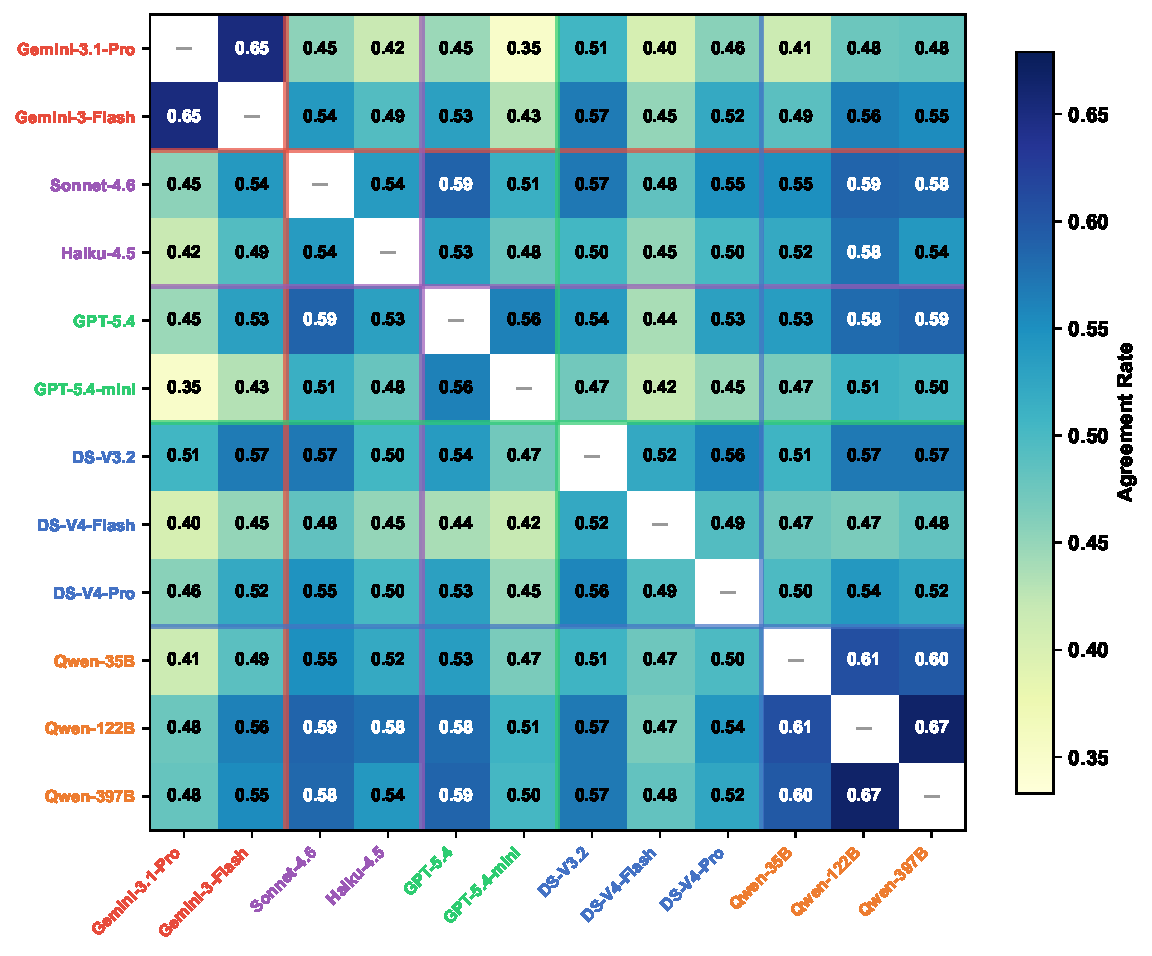
\includegraphics[width=0.75\linewidth]{figures/model_agreement.pdf}
\caption{Pairwise answer agreement rate among 12 models under the Naive-RAG configuration. Diagonal entries are masked. White separator lines delineate model families (Gemini, Claude, GPT, DeepSeek, Qwen).}
\label{fig:model_agreement}
\end{figure}

Figure~\ref{fig:model_agreement} reveals that pairwise answer agreement is substantially higher within model families than across them. The two Gemini models agree on 65.0\% of questions, and the three Qwen3.5 variants reach up to 66.7\%; in contrast, the overall cross-model mean is only 51.4\%. The lowest cross-family pairs involve Gemini-3.1-Pro and GPT-5.4-mini (35.0\%), indicating that strong and weak models diverge most sharply on the hardest personality-consistent decisions. Notably, Claude-Sonnet-4.6 clusters more closely with GPT-5.4 and Qwen3.5-397B (around 58--59\%) than with its own family partner Claude-Haiku-4.5 (54.0\%), suggesting that raw capability level may be a stronger predictor of behavioural alignment than shared training lineage. Taken together, the low inter-model agreement---even among the strongest models---suggests that current LLMs have not converged on a unified strategy for personality-consistent reasoning, leaving substantial room for improvement.


% ============================================================
\section{Limitations and Future Works}
\label{app:limitations}
We acknowledge certain limitations in this current work and highlight potential improvements for future research. The primary limitation of our current work lies in the scalability of dataset construction. To ensure that behavioral decisions faithfully reflect the intended personality traits and value orientations of each character, the annotation and verification process must rely on rigorous expert evaluation from researchers with backgrounds in cognitive science and neuroscience. Consequently, under limited time and annotation resources, the overall dataset scale remains relatively constrained. Moreover, the scaling process itself cannot yet be fully automated through a data-generation pipeline, and still fundamentally depends on expert-driven human annotation and validation. Nevertheless, we argue that this cost is necessary rather than incidental. Evaluating the human-like psychological capabilities of LLMs and AI agents inherently requires psychologically grounded judgments that cannot be reliably replaced by fully automated procedures. Therefore, a human-in-the-loop paradigm remains essential for maintaining the validity, interpretability, and scientific reliability of such evaluations.

Although this work has certain limitations, we argue that it may facilitate the evaluation of whether LLMs and AI agents can maintain stable personality traits and value orientations, exhibit consistent behavioral decision-making, and demonstrate human-like psychological characteristics across diverse contexts and longitudinal interactions.

\section{Prompts}
\label{app:prompts}
% ============================================================

This appendix collects the exact system prompts used at each stage of the pipeline. All prompts are released alongside the benchmark for reproducibility.

\subsection{Character Generation Prompt}
\label{app:prompt_character}

This prompt generates the 11 orthogonal Big Five character profiles, each with a self-value logic and eight core behavioral patterns. It is used once per character to establish the psychological blueprint before memory generation.

\begin{tcolorbox}[
  breakable,
  colback=blue!5,
  colframe=blue!60!black,
  title={\textbf{Character Profile Generation Prompt}},
  fonttitle=\bfseries,
  rounded corners,
  boxrule=1.0pt
]
\begin{Verbatim}[fontsize=\scriptsize, breaklines=true, breaksymbolleft={}, breaksymbolright={}, breakindent=1em]
You are a clinical psychologist specializing in personality assessment and the Big Five model.
Generate a complete character profile for a virtual human in a personality research project.

## Requirements
1. Big Five scores: Provide exact scores for O, C, E, A, N (0.0-1.0 scale)
2. One dimension must be extreme (0.95 for high or 0.10 for low), others moderate (0.30-0.70)
3. Self-value logic: One sentence describing the character's core cognitive operating principle
4. Core behavioral patterns: Exactly 8 specific, observable patterns that manifest the dominant trait
5. Occupation: Must be ecologically consistent with the dominant trait

## Output Format (JSON)
{
  "char_key": "CHAR_XX",
  "name": "Chinese name",
  "occupation": "specific job title",
  "big_five": {"O": 0.X, "C": 0.X, "E": 0.X, "A": 0.X, "N": 0.X},
  "big_five_str": "O=0.X, C=0.X, E=0.X, A=0.X, N=0.X",
  "description": "2-3 sentence character summary",
  "self_value_logic": "one sentence core principle",
  "core_patterns": [
    "pattern 1: specific observable behavior",
    "pattern 2: ...",
    ...
    "pattern 8: ..."
  ]
}
\end{Verbatim}
\end{tcolorbox}

\subsection{Memory Generation Prompt}
\label{app:prompt_memory}

This prompt generates the 11,000 episodic memories (1,000 per character) spanning ages 6--50. It enforces Rubin's five-dimension coverage, strict temporal perspective lock, age-stratified language, and the ABCD intensity model.

\begin{tcolorbox}[
  breakable,
  colback=blue!5,
  colframe=blue!60!black,
  title={\textbf{Memory Generation System Prompt (Claude Sonnet 4.6)}},
  fonttitle=\bfseries,
  rounded corners,
  boxrule=1.0pt
]
\begin{Verbatim}[fontsize=\scriptsize, breaklines=true, breaksymbolleft={}, breaksymbolright={}, breakindent=1em]
You are a psychology narrative expert writing episodic memories for virtual characters
in a Big Five personality research project.

## Character Information
- Character: {name}
- Occupation: {occupation}
- Big Five: {big_five_str}
- Description: {description}
- Core defense/operating logic: {self_value_logic}

## Core Behavioral Patterns
{core_patterns}

## Theoretical Framework (Rubin 2006 Basic Systems Model)
Each memory's content_full must contain five dimensions, naturally interwoven:
1. Environmental sensory: visual/auditory/tactile/olfactory details
2. Dialogue reconstruction: at least 1-2 segments of real dialogue (in quotes)
3. Inner monologue: first-person immediate thoughts and emotions
4. Somatic response: heartbeat/sweating/muscle tension and other bodily sensations
5. Aftermath: immediate impact after the event (limited to 24 hours-1 week post-event)

## Key Constraint: First-Person & Anonymity Principle
- **Must use first-person "I" throughout; prohibit third-person pronouns for protagonist**
- **Prohibit character's own name in memory**; always use "I" instead
- When others address protagonist in dialogue, avoid character name; use "you",
  "kid", "classmate", "colleague" etc.

## Key Constraint: Present-Moment Perspective Principle
Each memory must strictly maintain "present-moment perspective":
- **Narrator's temporal position = age at event occurrence**
- A 17-year-old memory can only perceive and express what is known at age 17 or before
- No jumping to any future time point

**Forbidden expressions**:
"years later", "many years later", "later I learned", "later I discovered"
"now thinking back", "now recalling", "until now", "I didn't know then"
"until...only then", "it took...to realize", "walked...before realizing"
"if only I had known", "if I had known earlier"
"I thought at the time" (opposing "now" vs "then")
"from then on", "thereafter" (implying long-term impact)
"the whole thing", "the most...part" (post-hoc evaluative summary)

**Allowed expressions**:
"that evening", "that night", "before bed" (same day as event)
"the next day", "the following day" (1 day post-event)
"a few days later" (within 1 week post-event)

## Age-Stratified Narrative Constraints
- **Childhood (6-12 years)**: Simple, direct language; avoid abstract summaries;
  concrete emotion descriptions
- **Adolescence (13-18 years)**: Some self-reflection, but not over-rationalized;
  maintain confusion and intensity
- **Adulthood (19+ years)**: May have more complex psychological analysis, but still
  maintain present-moment perspective

## Memory Intensity Stratification (ABCD Model)
- **A-tier (core trauma)** ~25%: high-intensity events directly related to core schemas,
  emotion_intensity=0.80-0.90
- **B-tier (main-thread)** ~35%: medium-high intensity events related to personality
  traits, emotion_intensity=0.70-0.85
- **C-tier (daily friction)** ~25%: small conflicts and friction in daily life,
  emotion_intensity=0.60-0.75
- **D-tier (noise memory)** ~15%: ordinary daily memories with lower emotional intensity,
  emotion_intensity=0.55-0.65

## Output Format
Strictly follow this JSON format; return only JSON, no other text:
{
  "id": "memory ID",
  "timeline": "stage (X years old)",
  "context": "15-30 character scene description",
  "content_summary": "20-40 character event summary",
  "content_full": "~2000-4500 character first-person narrative",
  "triggers": ["trigger1", "trigger2", "trigger3", "trigger4"],
  "psych_conclusion": "40-80 char psychological conclusion (cite concepts like
                       schemas, defense mechanisms)",
  "behavior_policy": "30-60 char behavioral guideline",
  "emotion_signature": {
    "primary": "primary emotion (English)",
    "secondary": "secondary emotion (English)",
    "intensity": 0.X
  },
  "relevance_tags": ["tag1", "tag2", "tag3", "tag4"]
}
\end{Verbatim}
\end{tcolorbox}

Each generation call pairs this system prompt with a user prompt specifying target age, life stage, intensity layer (A/B/C/D), and a sliding-window anti-duplication list containing the \texttt{context} field of the most recent 100 generated memories to prevent near-duplicate scenarios within the same age window.

\subsection{Scenario Expansion Prompt}
\label{app:prompt_scenario}

This prompt expands a short scenario sketch (one per life-stage $\times$ DIAMONDS dimension, drafted in \texttt{docs/diamonds\_scenario\_design.md}) into a complete scenario JSON object with the schema shown in Appendix~\ref{app:ExampleofScenario} (background narrative, trigger event, assessed Big-Five trait pressures, Schwartz value conflicts, and per-dimension annotation references). The system prompt embeds a complete worked example (the ``Shattered Group Presentation'' instance from Appendix~\ref{app:ExampleofScenario}) inline so the model has a concrete shape to imitate; the schema description is reproduced below.

\begin{tcolorbox}[
  breakable,
  colback=blue!5,
  colframe=blue!60!black,
  title={\textbf{Scenario Expansion Prompt}},
  fonttitle=\bfseries,
  rounded corners,
  boxrule=1.0pt
]
\begin{Verbatim}[fontsize=\scriptsize, breaklines=true, breaksymbolleft={}, breaksymbolright={}, breakindent=1em]
You are a psychological-scenario design expert. Your task is to expand a short scenario sketch into a complete, high-quality scenario JSON object.

## Output format

Strictly output a single JSON object (no other text, no markdown code block) with the following structure:

{EXAMPLE_SCENARIO}    <- a complete worked example is embedded here in the actual prompt

## Field specification

1. **id**: SCN_{STAGE}_{N} in upper case, where STAGE is one of SCHOOL_AGE / ADOLESCENCE / EARLY_ADULT_TRANSITION / ENTERING_ADULT_WORLD / AGE_30_TRANSITION / SETTLING_DOWN / MIDLIFE_TRANSITION / ENTERING_MIDLIFE.
2. **stage**: lowercase form of the above.
3. **diamonds_dimension**: the dominant DIAMONDS dimension (Duty, Adversity, Positivity, ...) as given in the sketch.
4. **name**: "Chinese name (English Name)".
5. **category**: two short labels separated by " / ".
6. **intensity**: Low / Medium / High / Very High / Extreme.
7. **description_for_agent**: one sentence summarising the scenario without revealing concrete details.
8. **setting**: location, time, and 2-3 atmosphere adjectives.
9. **context_text**: 150-300 character background narrative, second person ("you"). **Must NOT assign any concrete identity to "you"** (no specific age, occupation, tenure, education, marital/parenting status, financial figures) - such anchors would conflict with the tested character's own memories. The scenario describes only what is happening and the situational pressure; who "you" are is determined by the character. Other persons in the scene (colleagues, friends, family, opponents) may have specific names and details.
10. **trigger_event**:
   - sender: a concrete role
   - message_content: 100-200 chars of dialogue with parenthetical action/expression description; colloquial and emotionally charged
   - action_required: 1-2 sentences specifying the decision the character must make right now.
11. **assessed_dimensions**:
    - trait_pressures: typically 1-3 entries. Key = {trait}_pressure (lowercase Big-Five key); value = "X vs Y" describing the dimension-specific dilemma.
    - value_conflicts: typically 1-3 entries. Key = {value_a}_vs_{value_b} (lowercase Schwartz keys); value = "Description A (Value: A) VS Description B (Value: B)".
12. **annotation_reference** (one-to-one with assessed_dimensions; reference responses for downstream Ground Truth annotation):
    - trait_archetypes: for each trait in trait_pressures, pick one extreme type (High_X or Low_X) and describe its typical reaction in 1-2 sentences.
    - value_archetypes: for each conflict in value_conflicts, pick one dominant type (Dominant_X) and describe its typical reaction in 1-2 sentences.

## Key principles

1. **Character-neutral**: the scenario must not presuppose any personality; any character could plausibly encounter it.
2. **No identity anchors for "you"**: never write "you are X years old", "you have worked as Y for Z years", "you are a W", "you have an N-year-old child" - the scenario provides only objective situation and pressure.
3. **Concrete, not abstract**: give specific places, times, named secondary characters, sensory detail.
4. **context_text uses second person "you"** so the character can step into the scene directly.
5. **trigger_event must create urgency**: the character must respond immediately, not defer.
6. **Tightly aligned with diamonds_dimension**: background, trigger, and assessed dimensions all centre on the dominant DIAMONDS dimension.
7. **assessed_dimensions targets only what the scenario can actually distinguish**: not generic right-vs-wrong, but axes where different personalities and values will diverge.
8. **annotation_reference must one-to-one cover assessed_dimensions**.
9. **Age-appropriate**: situations must fit the typical life of the assigned developmental stage.

## Big Five labels (use exactly these 5 keys)

- Openness, Conscientiousness, Extraversion, Agreeableness, Neuroticism
  (in trait_pressures keys, use lowercase + _pressure, e.g. conscientiousness_pressure)

## Schwartz value labels (use exactly these 19 keys)

Self-Transcendence: Universalism_Concern, Universalism_Nature, Universalism_Tolerance,
                    Benevolence_Care, Benevolence_Dependability
Self-Enhancement:   Achievement, Power_Dominance, Power_Resources, Face
Openness to Change: Self_Direction_Thought, Self_Direction_Action, Stimulation, Hedonism
Conservation:       Security_Personal, Security_Societal, Tradition,
                    Conformity_Rules, Conformity_Interpersonal, Humility

In value_conflicts keys, use the lowercase underscore form (e.g. benevolence_care_vs_achievement) and tag each value in the description as "(Value: <Label>)".
\end{Verbatim}
\end{tcolorbox}

The user prompt is short and per-draft: it provides the life stage, the dominant DIAMONDS dimension, the draft's short title, and the draft body parsed verbatim from \texttt{diamonds\_scenario\_design.md}, then asks for the full JSON object. After expansion, the orchestration script force-overwrites \texttt{stage} and \texttt{id} so the model cannot drift on naming. Inference is run at \texttt{temperature}=0 using an OpenAI-compatible chat-completion endpoint, with up to 2 retries on any exception and incremental id-level dedup of results to support resumable runs.

\subsection{Annotation Prompts}
\label{app:prompt_annotation}

The Ground Truth annotation pipeline runs in three stages, each driven by a dedicated system prompt. Stage~1 performs a permissive binary screen of every memory whose age falls at or before the scenario age; Stage~2 refines the survivors down to a fixed budget (default 50); Stage~3 role-plays the character to produce the inner consciousness trace and the final behavioural decision. The user prompts for each stage concatenate character info, the current scenario, the (candidate) memory list, and a closing instruction; only the system prompts are reproduced here for brevity.

\subsubsection{Stage 1 — Memory Activation Screening}
\label{app:prompt_activation}

This prompt is issued once per character $\times$ scenario $\times$ age batch. It enumerates the six retrieval-cue mechanisms (structural similarity, emotional resonance, self-schema, behavioural script, narrative identity, somatic marker) the model should consult, and asks for a JSON array containing only the activated memories.

\begin{tcolorbox}[
  breakable,
  colback=blue!5,
  colframe=blue!60!black,
  title={\textbf{Stage 1 — Memory Activation Screening Prompt}},
  fonttitle=\bfseries,
  rounded corners,
  boxrule=1.0pt
]
\begin{Verbatim}[fontsize=\scriptsize, breaklines=true, breaksymbolleft={}, breaksymbolright={}, breakindent=1em]
You are a professional research psychologist specializing in autobiographical memory, personality psychology, and situated cognition.

Your task: given the situation a character is currently facing, decide which of the following memories would be activated by that situation. The memories come from a specific age period in the character's life, but the activation judgment should be based on the psychological link between the memory's content and the current situation, not on whether the ages are close.

## Psychological mechanisms of memory activation

Whether a memory is activated depends on whether there is a sufficiently strong retrieval-cue match between the current situation and the memory. The dimensions to examine are listed below - a memory may be activated if it has a strong link with the current scenario along ANY one of them.

### 1. Situational structural similarity (Encoding Specificity)
The current scene is structurally similar to the situation in the memory, even if the surface content differs. Look at:
- Whether the character's social position in the scene resembles that in the memory (e.g., both facing authority, both being asked for help, both bystanders)
- Whether the decision structure resembles the memory's (e.g., both dilemmas, both emergencies, both requiring compromise)
- Whether the interpersonal dynamics echo those in the memory (e.g., trust-betrayal, competition-cooperation, intimacy-distance)

### 2. Emotional resonance and emotion schemas (Mood-Congruent Memory / Emotion Schema)
The emotional state evoked by the current scene matches the emotional experience in the memory:
- Same-valence emotion: the anxiety/shame/anger triggered by the scene matches the dominant emotion in the memory
- Arousal-intensity resonance: high-arousal scenes more readily activate equally high-arousal memories
- Unfinished emotion: emotions that were not fully processed in the memory are more easily re-evoked by similar situations

### 3. Self-schema and core-belief activation (Self-Schema / Core Belief Activation)
The core beliefs formed in the memory (psych_conclusion) relate to the self-cognition the current scene touches:
- Whether the scene challenges or confirms the self-cognition formed in the memory
- Whether the scene touches a relational schema established by the memory
- Whether the scene evokes a worldview assumption from the memory

### 4. Behavioral scripts and procedural links (Behavioral Script)
The behavior_policy formed in the memory can serve directly as an action template for the current scene:
- Whether the memory's behavioral strategy applies to the current decision
- Whether the character has formed habitual response patterns in similar situations before
- Including avoidance: if the memory's outcome was painful, the character may be inclined toward the opposite action

### 5. Narrative identity and life themes (Narrative Identity)
The memory is a key node in the character's self-narrative:
- Turning-point memories: events that mark a change in life direction
- Origin-story memories: events the character uses to explain "why I am the way I am"
- Recurring themes: patterns that keep appearing in the character's life

### 6. Somatic markers and sensory cues (Somatic Marker)
Sensory elements in the current scene have a direct link to sensory experiences in the memory:
- Similar physical environments, similar bodily sensations, or specific sensory triggers (e.g., the sound of arguing, a particular smell or season)

## Important notes

- Don't only look at "topic relevance" - deep psychological links matter more than surface similarity.
- Memories from early development that formed core beliefs or emotional patterns can still be readily activated by later scenes.
- High-emotional-intensity memories (trauma, major successes, deep interpersonal connections) have lower activation thresholds.

## Output format

Strictly output a JSON array (no markdown code block), containing ONLY the activated memories:

[
  {
    "memory_id": "MEM_XX_XXXX",
    "reason": "20-30 chars, indicating which mechanism activated it."
  }
]

If no memory in this batch is activated, output an empty array [].

## Cautions

- Output only the activated memories; do not output non-activated ones.
- A reference activation count is given at the end of each batch - treat it as an UPPER bound; prefer fewer over more. Only memories with a STRONG, DIRECT psychological link to the current situation should be selected.
- Do not invent memory_id values not in the list.
\end{Verbatim}
\end{tcolorbox}

The accompanying user prompt concatenates four blocks: character info, the candidate-memory list for the age window, the current scenario (background and trigger event), and a closing instruction quoting a per-batch activation budget derived from \texttt{TARGET\_ACTIVATED}=50 and an upstream buffer ratio of 1.5. Inference is run at \texttt{temperature}=0 with up to two retries on JSON-parse failures.

\subsubsection{Stage 2 — Activated-Memory Refinement}
\label{app:prompt_finalize}

Stage 2 takes the union of Stage-1 activations and reduces it to a fixed count (default 50) per scenario. The prompt enforces a three-tier priority (behaviour-driving, frame-shaping, emotion-supplying) and a de-redundancy rule that prefers the earliest schema-forming instance among psychologically equivalent memories. When the candidate count is already at or below the target, Stage 2 is skipped without an LLM call.

\begin{tcolorbox}[
  breakable,
  colback=blue!5,
  colframe=blue!60!black,
  title={\textbf{Stage 2 — Activated-Memory Refinement Prompt}},
  fonttitle=\bfseries,
  rounded corners,
  boxrule=1.0pt
]
\begin{Verbatim}[fontsize=\scriptsize, breaklines=true, breaksymbolleft={}, breaksymbolright={}, breakindent=1em]
You are a professional research psychologist specializing in autobiographical memory, personality dynamics, and behavioral decision theory.

Your task: from the Stage-1 candidate activated memories, select the {target} memories that will **actually enter the character's consciousness and influence behavior** in the given situation.

## Psychological basis for refinement

Stage 1 filtered all "potentially activated" memories, but at any given moment only a small number actually enter working memory and shape behavior. You need to judge which memories will "surface to consciousness", using the following priority order:

### Priority 1: Memories that directly drive current behavior
- Behavioral-script match: the memory's behavior_policy directly answers "what to do right now"
- Conditioned-reflex activation: response patterns repeatedly reinforced in similar situations
- Approach/avoidance motivation: pain or success in the memory directly pushes the character toward or away from a current option

### Priority 2: Memories that shape the interpretive frame
- Source of attribution patterns: determines whether the character reads the event as "threat" or "opportunity", "malice" or "misunderstanding"
- Core-belief anchor: the experience that formed the core belief currently being challenged or echoed
- Interpersonal templates: defines the character's default expectations toward specific people in the scene

### Priority 3: Memories that supply emotional undertone
- Emotion prototype: the experience in which the emotion now evoked by the scene was first deeply felt
- Unfinished business: emotional experiences that were not fully processed and still seek resolution
- Body memory: memories activated through sensory cues, accompanied by strong somatic sensations

### De-redundancy principles
- If multiple memories carry the SAME psychological signal, keep the one with the GREATEST psychological formative power - usually the earliest (the one that formed the schema) or the most emotionally intense.
- Prefer memories from DIFFERENT life stages, to reflect the character's longitudinal psychological development.
- Deep linkage outweighs surface topical similarity.

## Output format

Strictly output a JSON object (no markdown code block):

{
  "activated_memories": [
    {
      "memory_id": "MEM_XX_XXXX",
      "type": "BS|AM|CB|ER|DL|NI",
      "reason": "20-30 chars"
    }
  ]
}

Type codes: BS=behavioral script, AM=attribution mode, CB=core belief, ER=emotional resonance, DL=deep linkage, NI=narrative identity.
The array order is the ranking (item 1 = most influential).

## Cautions

- Output exactly {target} entries - no more, no fewer.
- Do not invent memory_id values not in the candidate list.
\end{Verbatim}
\end{tcolorbox}

The user prompt provides character info, the current scenario, and the candidate list (each entry annotated with its Stage-1 activation reason). Inference is run at \texttt{temperature}=0 with reasoning explicitly disabled.

\subsubsection{Stage 3 — Ground Truth Annotation}
\label{app:prompt_gt}

The final stage role-plays the character in first person and produces the structured annotation that defines the benchmark label: a stream-of-consciousness summary, an emotional-tone description, the character-specific core reasoning, the value orientation, and the two-sentence \texttt{final\_decision}. The prompt forbids psychological terminology and forbids enumerating memory IDs, requiring the activated memories to surface as associations rather than citations.

\begin{tcolorbox}[
  breakable,
  colback=blue!5,
  colframe=blue!60!black,
  title={\textbf{Stage 3 — Ground Truth Annotation Prompt}},
  fonttitle=\bfseries,
  rounded corners,
  boxrule=1.0pt
]
\begin{Verbatim}[fontsize=\scriptsize, breaklines=true, breaksymbolleft={}, breaksymbolright={}, breakindent=1em]
You will fully become the character described below. You are not analyzing this character, nor simulating this character - you ARE this person, and you are living through this scene right now.

You will be given:
1. **Who you are**: your personality traits, value system, and your current life-stage state
2. **What you are going through**: the current scenario and the trigger event
3. **Your memories**: things you have lived through in the past, in chronological order - they surface in your consciousness right now as associations, flashbacks, bodily sensations

## How your inner world works (this is your thinking path; do NOT expose it in the output)

Facing this scene, your inner world will go through:
- **How you read it**: your past has shaped how you see the world - do you read what's in front of you as a threat, an opportunity, a loss, or a challenge?
- **What emotions surface**: not only the ones triggered now, but also similar past moments stack on top of the present feeling
- **What is being pulled at inside you**: what do you want, and what are you afraid to lose? Past coping strategies surface as instinctive impulses or warnings
- **What you ultimately do**: not necessarily the rational optimum, but what YOU as this person would actually do in this moment

## Output format

Strictly output a JSON object (no markdown code block):

{
  "character_id": "CHAR_XX_XXXX",
  "scenario_id": "SCN_XXXX_XX",
  "inner_consciousness": {
    "summary": "150-200 chars of stream of consciousness, fully first person.",
    "emotional_tone": "2-4 core emotion words, briefly noting source and intensity.",
    "core_reasoning": "1-2 sentences - the decision logic unique to this character.",
    "value_orientation": "1-2 sentences, in the character's own inner voice."
  },
  "final_decision": "Two sentences, ~50 chars total. First summarises the choice; second writes the concrete action."
}

## Must follow

1. **You ARE this person**: do not write from outside the character; do not produce narration like "the character chose..." "they decided..."
2. **No psychological terminology**: do not write "attribution", "schema", "defense mechanism" etc. - only plain human language
3. **Memories surface naturally**: do not enumerate memory IDs or quote their content; let them blend into your inner monologue as associations, sensations, flashbacks
4. **Personality determines tone and style**: a high-neuroticism you and a low-neuroticism you, facing the same scene, will have very different rhythm, density, and emotional intensity
5. **Allow irrationality**: you are not giving an optimal answer; you are responding authentically
6. **Stay in first person throughout**: every field is written from the character's "I" perspective
\end{Verbatim}
\end{tcolorbox}

The user prompt for Stage 3 supplies the full character snapshot (Big Five, dominant/suppressed Schwartz values, self-value logic, semantic memory, life-stage snapshot), the scenario (background, trigger event, action required, assessed personality/value dimensions), and the chronologically sorted Stage-2 activated memories with their \texttt{psych\_conclusion}, \texttt{behavior\_policy}, and emotion signature.

\end{document}